\documentclass[Master, ngerman, UKenglish]{scrbook}
%------------------------------------------------------------------------------
% This file contains a skeleton thesis for
% a Physics or Astronomy Institute in the University of Bonn

% Specify the thesis type as an option: PhD, Master, Diplom, Bachelor
% Specify the thesis stage as an option: Draft (default), Submit, Final, PILibrary

% Specify the language(s) in the class and then use babel.
% If you need more than one language, give the default language last,
% e.g. ngerman, UKenglish for a thesis in British (UK) English where you want
% to be able to set the language to German for some part of it.

%------------------------------------------------------------------------------
% Pass TeX Live version to the package
% Use command pdflatex --version to find out which version you are running
% Add option backref=false when your thesis is ready to turn off back-referencing
% in your bibliography
\usepackage[texlive=2020, biblatex=false]{ubonn-thesis}
% Adjustments to standard biblatex style
%\usepackage{ubonn-biblatex}
%\usepackage[backend=biber, style=nature, hyperref, doi=false, maxbibnames=5]{biblatex}
\usepackage[backend=biber, backref=true, doi=false, style=phys, biblabel=brackets, sorting=none, block=ragged, maxbibnames=5, firstinits]{biblatex}


% Glossary package
% \usepackage[acronym,toc,nosuper]{glossaries}
\usepackage{acro,hyperref,longtable,tabu}
% TikZ packages and libraries
% \usepackage{tikz}
% \usepackage{tikz-3dplot}
% \usepackage{pgfplots}
% \usetikzlibrary{positioning,shapes,arrows}
% \usetikzlibrary{decorations.pathmorphing}
% \usetikzlibrary{decorations.markings}
\usepackage{thesis_defs}
\usepackage{multirow}
\usepackage{physics}

%------------------------------------------------------------------------------
% Instead of colouring  links, cites, table of contents etc.
% put them in a coloured box for the screen version.
% This is probably a good idea when you print your thesis.
 \hypersetup{colorlinks=false,
   linkbordercolor=blue,citebordercolor=magenta,urlbordercolor=darkgreen
 }

%------------------------------------------------------------------------------
% When writing your thesis it is often helpful to have the date and
% time in the output file. Comment this out for the final version.
%\ifoot[\today{} \thistime]{\today{} \thistime}

% In order to check if your labels are referenced try the refcheck package
% \usepackage{refcheck}

%------------------------------------------------------------------------------
% biblatex is included by ubonn-thesis. Look there for the settings used.
% See the options for settings that can be changed easily.
% For further changes copy the \RequirePackage[...]{biblatex} here
% and include ubonn-thesis with the option biblatex=false.

% Specify the bibliography files here and not at the end!
% Use standard_refs-bibtex if you use bibtex or bibtex8
% and standard_refs-biber  if you use biber
\addbibresource{bib/thesis_refs.bib}
%\addbibresource{bib/standard_refs-biber.bib}

%------------------------------------------------------------------------------
% The following definitions are used to produce the title pages
% needed at various stages
\newcommand{\thesistitle}{Raman manipulation between momentum state components of ultracold erbium atoms}
\newcommand*{\thesisauthor}{Pedro Castro Perez}
\newcommand*{\thesistown}{Tremp (LLeida), Spain}
\renewcommand*{\InstituteName}{\IAP}
\renewcommand*{\inInstitute}{\inIAP}
\renewcommand*{\InstituteAddress}{\IAPaddress}
% Adjust \thesisreferee...text depending on male/female referee
\newcommand*{\thesisrefereeonetext}{1.\ Gutachter}
\newcommand*{\thesisrefereeone}{Prof.\ Dr.\ Martin Weitz}
\newcommand*{\thesisrefereetwotext}{2.\ Gutachter}
\newcommand*{\thesisrefereetwo}{Prof.\ Dr.\ Sebastian Hofferberth}
% Date when thesis was submitted (Master/Diplom)
% Year or Month, Year when thesis was submitted (PhD)
\newcommand*{\thesissubmit}{01.06.2021}
% \newcommand*{\thesissubmit}{Month 2020}
% Date of thesis examination (PhD)
\newcommand*{\thesispromotion}{XX.YY.2021}
% Month and year of the final printed version of the thesis
\newcommand*{\thesismonth}{Juli}
\newcommand*{\thesisyear}{2021}
\newcommand*{\thesisnumber}{BONN-IR-2021-XXX}

%------------------------------------------------------------------------------
% The abstract is only needed for the printed version and should be in
% English regardless of the language of the thesis
\newcommand{\thesisabstract}{%
  \begin{otherlanguage}{UKenglish}
    This is your thesis abstract. It may be in a language that is
    different from the rest of your thesis.
  \end{otherlanguage}
}

%------------------------------------------------------------------------------
% \includeonly can be used to select which chapters you want to process
% A simple \include command just inserts a \clearpage before and after the file
% Note that \includeonly can be quite picky! Do not forget to put a
% comma after the filename, otherwise it will simply be ignored!
 \includeonly{%
   1_thesis_intro,
   2_thesis_bec_condensation,
   3_thesis_bec_diffraction,
   4_thesis_raman_manipulation,
   5_thesis_results,
   6_outlook,
   %thesis_appendix,
   %thesis_acknowledge% <----------------------------------------------------------UNCOMMENT ACKNOWLEDGEMENTS!
 }

%------------------------------------------------------------------------------
% Give a list of directories where figures can be found. Do not leave
% any spaces in the list and end the directory name with a /
\graphicspath{%
  {figs/}%
  {figs/cover/}%
}

%------------------------------------------------------------------------------
% Make a list of acronyms
\acsetup{list/template=longtabu, list/heading=addchap}

\DeclareAcronym{bec}{short=BEC,long=Bose-Einstein condensate}
\DeclareAcronym{mot}{short=MOT,long=magneto-optical trap}
\DeclareAcronym{odt}{short=ODT,long=optical dipole trap}
\DeclareAcronym{ai}{short=AI,long=absorption imaging}
\DeclareAcronym{tc}{short=TC,long=transversal cooling}
\DeclareAcronym{zs}{short=ZS,long=zeeman slower}
\DeclareAcronym{ule}{short=ULE cavity,long=ultra low expansion cavity}
\DeclareAcronym{aom}{short=AOM,long=acousto-optic modulator}
\DeclareAcronym{ec}{short=EC,long=effusion cell}
\DeclareAcronym{hl}{short=HL,long=hot lip}
\DeclareAcronym{uhv}{short=UHV,long=ultra-high vacuum}
\DeclareAcronym{dfc}{short=DFC,long=dual filament effusion cell}
\DeclareAcronym{rms}{short=RMS,long=root mean squared}
\DeclareAcronym{quest}{short = QUEST, long = Quasi-electrostatic trap}
\DeclareAcronym{tof}{short = TOF, long = time of flight}
\DeclareAcronym{pbs}{short = PBS, long = polarizing beam spliter}
\DeclareAcronym{rf}{short = RF, long = radio frequency}


% Draft version - add the word DRAFT on the cover pages
\ifthenelse{\equal{\ThesisVersion}{Draft}}{%
  \usepackage{background}
  \ifthenelse{\texlive < 2013}{%
    \SetBgContents{DRAFT}
    \SetBgColor{blue!30}
  }{%
    \backgroundsetup{contents=DRAFT, color=blue!30}
  }
}

%------------------------------------------------------------------------------
\begin{document}

% Cover page of thesis - this is only needed for the printed final
% version to be submitted to the department library
% Do not use this page for thesis submission to the Prüfungsamt or Promotionsbüro!
\ifthenelse{\equal{\ThesisVersion}{PILibrary}}{%
  \typeout{Document \jobname, Info: PI library version of thesis}
  \input{../Template/cover/\ThesisType_Cover}
}{}

% Start counting pages from the title page
\frontmatter
% Dedication has to come before \maketitle
% \dedication{Dedicated to no one}

% Select the correct title page(s)
\ifthenelse{\equal{\ThesisType}{Unknown}}{%
  \typeout{Document \jobname, Error: Unknown thesis type - no title page printed}
}{%
  % Bachelor thesis only has one title page
  \ifthenelse{\equal{\ThesisType}{Bachelor}}{%
    \typeout{Document \jobname, Info: Bachelor thesis}
    \input{../Template/cover/\ThesisType_Title}
  }{%
    \ifthenelse{\equal{\ThesisVersion}{Final} \OR \equal{\ThesisVersion}{PILibrary}}{%
      % Final and PI library versions
      \typeout{Document \jobname, Info: Final version of a \ThesisType  thesis}
      \input{../Template/cover/\ThesisType_Final_Title}
    }{% Submission and draft versions
      \input{../Template/cover/\ThesisType_Submit_Title}
      \typeout{Document \jobname, Info: Draft/submission version of a \ThesisType  thesis}
    }
  }
}

\pagestyle{scrplain}

%------------------------------------------------------------------------------
% You can add your acknowledgements here - don't forget to also add
% them to \includeonly above
%%------------------------------------------------------------------------------
\chapter*{Acknowledgements}
\label{sec:ack}
%------------------------------------------------------------------------------

I would like to thank ...

You should probably use \texttt{\textbackslash chapter*} for
acknowledgements at the beginning of a thesis and
\texttt{\textbackslash chapter} for the end.

%%% Local Variables: 
%%% mode: latex
%%% TeX-master: "../Thesis"
%%% End: 
 % <----------------------------------------------------------UNCOMMENT ACKNOWLEDGEMENTS!

\tableofcontents

\mainmatter
\pagestyle{scrheadings}

% Turn off DRAFT for the following pages
\ifthenelse{\equal{\ThesisVersion}{Draft}}{%
  \ifthenelse{\texlive < 2013}{%
    \SetBgContents{}
  }{%
    \backgroundsetup{contents={}}
  }
}{}

%------------------------------------------------------------------------------
% Add your chapters here - don't forget to also add them to \includeonly above
% !TEX root = Thesis.tex

%==============================================================================
\chapter{Introduction}
\label{chap:intro}
%==============================================================================

The first theorization of an ultracold ensemble of atoms was performed by Satyendra Nath Bose and Albert Einstein in 1924 during a series of publications where the concept of what is today known as a \acf{bec} was developed \cite{Bose1924, Einstein1924, Einstein1925}. At the time, this was a new state of matter formed by bosonic particles occupying the energetic ground state macroscopically for close to absolute zero temperatures. It took more than 70 years to obtain this theorised state of matter in an experiment. The first \acp{bec} were generated in 1995 by several research groups for three different chemical elements: rubidium \cite{Davis1995}, sodium \cite{Anderson1995} and lithium \cite{Bradley1995}. The following years lead to a rising interest of this exotic state of matter due to their quantum properties that allow to describe the system of particles by using just the coherent wave function of a single-particle. Due to this, \acp{bec} for many other elements were achieved. Some examples are: alkali metals like strontium \cite{Stellmer2009}, and Lanthanides like ytterbium \cite{Takasu2003}, dysprosium \cite{Lu2011} and erbium \cite{Aikawa2012}. Even in non-atomic bosonic particles like photons \cite{Klaers2010}.

Nowadays, there has been increasing interest in the condensation of atoms belonging to the lanthanide group. This is due to two main reasons: the first one being the large magnetic moment that these elements normally have, which increases the effect of dipole-dipole interaction \cite{Aikawa2012,Baier2018}. The second reason will be more relevant for this experiment and is based on the fact that these atoms normally have a non-vanishing electronic angular momentum in their energetic ground state. For the case of erbium, the orbital angular momentum has a value of $L=5$ for the ground state. This allows to use Raman transitions between Zeeman sublevels of the ground state in the fine structure scheme. Increasing the available detuning ranges, which enables the possibility of using large values for the detuning. This reduces the photon scattering rates and increases the coherence times for the \ac{bec} \cite{Grimm2000}.

Raman manipulation permits the use of a method called phase imprinting, which generates synthetic magnetic fields and have been theorised to be achievable with lanthanide atoms \cite{cui2013synthetic}. If these synthetic fields were generated with enough strength, it would enable the fractional quantum Hall regime for neutral atoms. This could have mayor implications possibly enabling studies of topological quantum computation. The synthetic magnetic fields have already been observed as vortices structures inside the \ac{bec} for rubidium \cite{Lin2009}. However, the strength of these fields was limited by the coherence time of the available transitions in this element. As said, the use of erbium permits longer coherence times, which could generate larger synthetic magnetic fields and possibly enable the fractional quantum Hall regime.

This thesis aims to study an Raman manipulation set-up formed by two counter-propagating beams detuned with respect to the \SI{841}{\nano\meter} erbium transition. The main part will consists on the characterization of Raman transitions between the momentum space for the energetic ground state of erbium. This corresponds to the atomic \ac{bec} diffraction with the Raman beams forming and optical lattice. This results in the generation of different momentum orders, similar to the well-known process of light diffraction. After this, the main focus will be the achievement of Raman transitions into the spin-momentum configuration between different sublevels, generated by Zeeman splitting of the ground energy level of the erbium \ac{bec}. This achievement represents the ground work for the future realisation of strong enough synthetic fields to reach the fractional quantum Hall regime. However, in order to obtain the Raman manipulation of internal spin states, an additional experiment with \ac{rf} transitions was required. Its main purpose was to characterize and prepare the magnetic fields causing the Zeeman splitting of the ground state.

Therefore, the thesis it is divided in different chapters according to its content. Chapter \ref{chap:erbium_bec} shows the properties of erbium, introduces the basic theory of an atomic \ac{bec} and briefly describes the experimental set-up used to achieve and measure an erbium \ac{bec}. Chapter \ref{chap:one_dimensional_lattices} gives the theoretical basis for the diffraction of a \ac{bec} with an optical lattice. Chapter \ref{chap:raman_manipulation} describes the \ac{rf} transitions experiment together with a basis of the Raman manipulation of the spin-momentum space. Chapter \ref{chap:results_and_discussion} shows the measured and analysed results. And finally, \ref{chap:outlook} serves as a conclusion and outlook to the thesis.

%%% Local Variables: 
%%% mode: latex
%%% TeX-master: "Thesis"
%%% End: 

% !TEX root = Thesis.tex

%==============================================================================
\chapter{Erbium \acl*{bec}}
\label{chap:erbium_bec}
%==============================================================================

This chapter has the objective of briefly review some relevant properties of Erbium, which will clarify what makes it relevant in the study of ultra cold atoms. After this, the basic theory of Bose-Einstein condensation will be discussed, along with a brief description of the experimental phases required to create and observe an erbium \ac{bec}. This experimental realization will be the foundation on which the following chapters will be grounded when discussing further experimental achievements.

%==============================================================================
\section{Properties of erbium} \label{sec:erbium_properties}
%==============================================================================
Erbium is a chemical element with an atomic number of 68, which belongs to the series of the Lanthanides. It is also part of the group called Rare-earth elements and it was first discovered by G. Monsander in 1843 \cite{mosander1843xxx}. The name of ``Erbium'' comes from the name of the Swedish village of Ytterby, the place where it was extracted. At that time, the similarity of rare-earth metals' chemical properties made their distinction extremely difficult. For this reason, what G. Monsander thought to be pure Erbium oxide was in fact a mixture of different rare-earth metal oxides. The element is not obtained in a reasonably pure form until 1937 by W. Klemm and H. Bommer \cite{klemm1937bommer}.

Considering some basic properties of this element, under standard conditions erbium is in a solid state. It has a silver shining surface, which oxidizes with air contact. This rare-earth metal has a melting point of \SI{1802}{\kelvin} and boiling point of \SI{3136}{\kelvin}. As a result, to be able to work with a free atomic gas of erbium requires to heap up the solid erbium metal to high temperatures \cite{emsley1998}.

The number of stables isotopes of Erbium is 6 and they can be seen in Table \ref{tab:Isotopes_Erbium}. All of them are bosons with nuclear spin of zero, in exception of $^{\text{167}}\text{Er}$, which is a fermion with spin of 7/2. The chosen isotope for this experiment is $^{\text{168}}\text{Er}$ because of its bosonic nature (see Section \ref{sec:bose-einstein_condensation}), high abundance and favorable scattering properties.

\begin{table}[htbp] \centering
	\begin{tabular}{@{}c|c|c|c@{}}\hline
		Isotope                  & Abundance [\%]          & Atomic Mass [u] & Nuclear Spin [$\hbar$] \\ \hline\hline
		$\text{Er}^{\text{162}}$ &  0.14                   & 161.928775      & 0   \\
		$\text{Er}^{\text{164}}$ &  1.61                   & 163.929198      & 0   \\ 
		$\text{Er}^{\text{166}}$ & 33.60                   & 165.930290      & 0   \\
		$\text{Er}^{\text{167}}$ & 22.95                   & 166.932046      & 7/2   \\
		$\text{Er}^{\text{168}}$ & 26.80                   & 167.932368      & 0   \\  
		$\text{Er}^{\text{170}}$ & 14.90                   & 169.935461      & 0   \\  \hline
	\end{tabular}
	\caption[Table with the stable isotopes of Erbium]{Table with the stable isotopes of Erbium that can be found on Nature with their respective Abundance ratio, Atomic mass and Nuclear Spin. Spectroscopy data taken from \cite{sansonetti2005handbook}.}\label{tab:Isotopes_Erbium}
\end{table}

In addition to these properties, erbium atoms have a rather complex energetic level scheme due to its open 4f shell. This one lacks 2 electrons to be completely filled, which makes erbium to have an electronic ground state with an orbital angular momentum value of $L = 5$ and a high magnetic moment of seven Bohr magneton $7\mu_B$ \cite{ban2005laser}. This high value for the orbital angular momentum in the ground state of erbium provides several advantages for Raman-coupling processes. Leading to longer coherence times and stronger synthetic magnetic fields when comparing with other alkali metals like rubidium or cesium, commonly used in ultracold atoms experiments  \cite{cui2013synthetic}.


A scheme of erbium energy levels together with the atomic transitions used in this experiment can be seen in figure \ref{fig:erbium_scheme}. The scheme shows that the electronic ground state of erbium is $\text{[Xe] }\text{4f}^{12} \text{6s}^2$, where [Xe]
represents the complete electronic configuration of Xenon\footnote{$\text{[Xe] = }\text{1s}^2 \text{ 2s}^2 \text{ 2p}^6 \text{ 3s}^2 \text{ 3p}^6 \text{ 3d}^{10} \text{ 4s}^2 \text{ 4p}^6 \text{ 4d}^{10} \text{ 5s}^2 \text{ 5p}^6$}. Moreover, the used optical transitions are represented by colored arrows in the figure and its spectroscopic data is shown in table \ref{tab:Transitions}. From now on, these three transitions will respectively be referred to as the 401nm, 583nm, and 841nm transitions.

Finally, it must be noted that aside from the discussed application in ultracold atoms, erbium is used in multiple commercial applications. One prominent example is the use or erbium as a fiber amplifier in doped silicon fibers \cite{mears1987low}. Furthermore, in nuclear physics it is used as neutron absorbing control rods \cite{emsley2011nature}.

%\sisetup{per-mode = symbol}%

\begin{table}[htbp] \centering
	\begin{tabular}{@{}l|c|c|S|S|S@{}}\hline
		\multicolumn{3}{c|}{Parameters} & \multicolumn{3}{c}{Transitions} \\ \hline
		Name & Symbol & Unit & \multicolumn{1}{c|}{401nm} & \multicolumn{1}{c|}{583nm} & \multicolumn{1}{c}{841nm} \\ \hline\hline
		Wavelength in vacuum & $\lambda$	& \si{\nano\meter}					& 400.91		& 582.84		& 841.22\\
		Lifetime 			& $\tau$	& \si{\micro\second}				& 0.045			& 0.857			& 20   \\ 
		Natural linewidth 	& $\Delta \nu_0$	& \si{\kilo\hertz}					& \num{33370} 	& 185.71 		& 7.96   \\
		Decay rate 			& $\gamma$	& \si{\per\second}					& \num{2.22e8} 	& \num{1.17e6}  & \num{5.00e4} \\
		Saturation intensity & $I_{S}$	& \si{\milli\watt\per\centi\meter}	& 71.80			& 0.12			& 1.74  \\  
		Doppler temperature	& $T_D$	& \si{\micro\kelvin} 				& 848.69  		& 4.46  		& 0.19    \\  
		Doppler velocity	& $v_D$	& \si{\centi\meter\per\second}		& 21.5 			& 1.49 			& 0.31 \\
		Recoil temperature	& $T_R$	& \si{\nano\kelvin} 				& 354.95  		& 167.94  		& 80.43    \\  
		Recoil velocity	& $v_R$	& \si{\milli\meter\per\second}		& 5.93 			& 4.08 			& 2.82 \\  \hline
	\end{tabular}
	\caption[Spectroscopic data for the optical transitions of Erbium]{Spectroscopic data for the optical transitions of Erbium used in this experiment. These transitions are called the 401nm, 583nm, and 841nm transitions and can be seen in figure \ref{fig:erbium_scheme}. Shown spectroscopic data taken from \cite{mcclelland2006natural, lawler2010atomic, den2010radiative, ban2005laser, lipert1993isotope}}\label{tab:Transitions}
\end{table}


\pagebreak


\begin{figure}[!htbp]\centering
	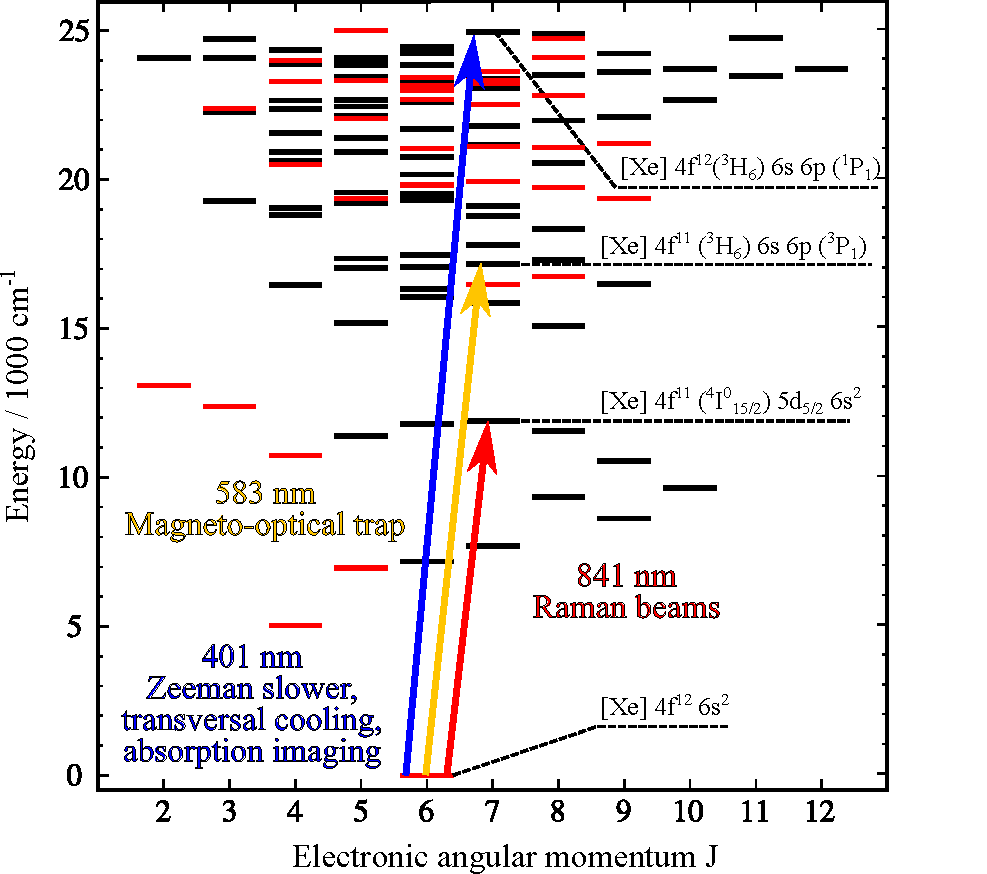
\includegraphics[width=1.\columnwidth]{erbium_term_scheme.pdf}
	\caption[Erbium energy scheme]{Energy level scheme of Erbium represented as a function of the total angular momentum J. This scheme shows only a range of energies relevant for the experiment of up to 25000 $\text{cm}^{\text{-1}}$. The different arrows show us the used transitions and for which phase of the experiment they are used for. The red lines represent energy states with even parity and the black lines those with odd parity. Data taken from \cite{NIST}. }\label{fig:erbium_scheme}
\end{figure}


%==============================================================================
\section{Bose-Einstein Condensation} \label{sec:bose-einstein_condensation}
%==============================================================================

A \ac{bec} is generally defined as a state of matter formed when a gas of bosons with a low density is cooled to near-zero temperatures (typically a few hundreds nanokelvins). To understand this definition and the next theoretical principles is necessary to define what is a Boson. In quantum mechanics, bosons are particles with an integer value in their spin. Because of this,  also have a symmetric wave function under the interchange of two particles, which allows bosons to have the same quantum state. Unlike its counterpart fermions, which have a half odd integer spin and an anti-symmetric wave function. Leading to Pauli's exclusion principle that avoids more than one fermion to occupy the same quantum state \cite{Pauli1925}.

It was the Indian physicist S. N. Bose in 1924, the first one who described in a successful way an ideal gas of non interacting free photons, behaving like mass-less bosons. His idea was initially rejected for publication in scientific journals. However, Bose sent the manuscript to A. Einstein, who recognized its importance, translated the paper to german and saw to it that was published \cite{Bose1924}. After this, Einstein extended Bose's treatment to massive particles and predicted the occurrence of a phase transition in a gas of non-interacting atoms, what is today known as a \ac{bec} \cite{Einstein1924, Einstein1925}.

These publications led to Bose-Einstein statistics, a model that explains the energetic behavior of a non-interacting gas of indistinguishable $N$ bosons, each one with mass $M$. The average number of particles at a given non-degenerate state with wave vector $\mathbf{k}$ and energy $E_\mathbf{k} = \hbar^2 \mathbf{k}^2 / 2M$ is given by

\begin{equation}\label{eq:bose-einstein_distribution}
	\bar{N}_{\mathbf{k}} = \frac{1}{e^{(E_\mathbf{k} - \mu)/k_B T} - 1}
\end{equation}
For an ideal gas of bosons in thermal equilibrium at a temperature $T$, Boltzmann constant $k_B$ and chemical potential $\mu$, which depends of $N$ and $T$ \cite{Masahito2010}. This relation can be expressed as

\begin{equation}\label{eq:chemical_potential_relation}
N = \sum_{\mathbf{k}}\frac{1}{e^{(E_\mathbf{k} - \mu)/k_B T} - 1}
\end{equation}

So the chemical potential $\mu$ is determined such that Eq. \eqref{eq:chemical_potential_relation} is satisfied for any given $N$ remaining constant. Now, expanding into the thermodynamic limit where $N$ and the occupied volume $V$ are increased to infinite values keeping the particle density $n = V/N$ constant. The sum over $\mathbf{k}$ appearing in Eq. \eqref{eq:chemical_potential_relation} can be replaced by an integral such as

\begin{equation}\label{eq:thermodynamic_limit}
n = \frac{N}{V} =  \frac{1}{(2\pi)^3}\int d^3 k\frac{1}{e^{(E_\mathbf{k} - \mu)/k_B T} - 1}
\end{equation}

For decreasing values of $T$ and constant $n$, the chemical potential increases becoming zero at a critical temperature $T_C$. By making $\mu = 0$, $T = T_C$ and $E_\mathbf{k} = \hbar^2 \mathbf{k}^2 / 2M$ in Eq. \eqref{eq:thermodynamic_limit} results

\begin{equation}\label{eq:thermodynamic_limit_at_critical_conditions}
n =  \zeta(3/2) \bigg(\frac{M k_B T_C}{2 \pi \hbar^2}\bigg)^{3/2}
\end{equation}
Where $\zeta(3/2) \simeq 2.612$ denotes the Riemann zeta function evaluated at 3/2. So the critical temperature of the \ac{bec} is given by

\begin{equation}\label{eq:critical_temperature}
T_C = 3.31 \frac{\hbar^2 n^{2/3}}{k_B M}
\end{equation}

A relevant case of study is when $T < T_C$ because a fraction of the $N$ bosons remains in the ground state with an energy $E = 0$. So the ideal gas of bosons can be divided in two energetic groups $N = N_{E=0} + N_{E>0}$. It must be noted that, the replacement of a sum by an integral in Eq. \eqref{eq:thermodynamic_limit} can only be take place in group of particles with an energy greater than zero $E>0$. As a result of this, the integral of Eq. \eqref{eq:thermodynamic_limit} for the case $T < T_C$ results

\begin{equation}\label{eq:thermodynamic_limit_low_T}
\frac{N_{E>0}}{V} = \zeta(3/2) \bigg(\frac{M k_B T}{2 \pi \hbar^2}\bigg)^{3/2}
\end{equation}

Using now equations \eqref{eq:critical_temperature}, \eqref{eq:thermodynamic_limit_at_critical_conditions} and the fact that $N_{E>0} = N - N_{E=0}$ results in an expression of the relative population of a \ac{bec} in an ideal bosons gas as a function of temperature:

\begin{equation}\label{eq:bec_relative_population}
\frac{N_{E=0}}{N} = 1 - \bigg(\frac{T}{T_C}\bigg)^{3/2}
\end{equation}

An intuitive way to think about this is to imagine the bosons as wave packets with a size of the thermal de Broglie length $\lambda_{th}$. This parameter is conventionally defined \cite{deBroglie1970}.

\begin{equation}\label{eq:de_Broglie_length}
\lambda_{th} = \frac{h}{\sqrt{2\pi Mk_B T}}
\end{equation}

For falling temperatures, the thermal de Broglie length begins to increase and the wave packets representing the bosons become greater in size. At $T\lesssim T_C$ the particles begin to occupy macroscopically the ground state and its wave packets start to overlap forming a macroscopic wave function, capable of describing the whole particle system. This is one of the most relevant properties of a \ac{bec}.

Now, we combine equations \ref{eq:thermodynamic_limit_at_critical_conditions} and \ref{eq:de_Broglie_length} obtaining

\begin{equation}\label{eq:phase_space_critical_point}
\qquad\qquad\qquad n \lambda_{th}^3 = \zeta(3/2) \simeq 2.612 \qquad \textrm{for } \ T=T_C
\end{equation}

The product of density with cubic de Broglie length is defined in literature as the phase-space density $\rho_{psd} \equiv n \lambda_{th}^3$. This parameter is normally used as a way of quantifying a given bosonic system. From Eq. \eqref{eq:phase_space_critical_point}, one can deduce that to form a \ac{bec} with an atomic (bosonic) cloud in three dimensions the phase space density must fulfill $\rho_{psd} \geq 2.612$. As a result, the required conditions to form a \ac{bec} can only be fulfilled when the atomic cloud is sufficiently cold and dense. For the case of a three dimensional gas of atoms trapped in an harmonic potential the condition over the phase space density is decreased to $\rho_{psd} \geq 1.2$ \cite{Pethick2008}. 

A further description about the theory of Bose-Einstein Condensation can be found in \cite{Masahito2010, Pethick2008}.

%==============================================================================
\section{Experimental realization of an erbium \ac{bec}} \label{sec:experimental_preparation}
%==============================================================================

To create experimentally a \ac{bec} of an atomic element such as erbium requires a multiple set of phases. Each one being based on different physical principles. The main purpose of this section is to discuss briefly every one of those together with its underlying foundation. For a more detailed description of the experimental set refer to  \cite{Ulitzsch2016}. 

Figure \ref{fig:table_set_up} shows a scheme of the experimental setup. It must be noted that all the devices used for the experiment lay on top of three optical tables represented in the figure by gray areas. Moreover, the laser beams produced by different laser systems are represented by colored lines. The erbium atoms are at all times kept inside an \ac{uhv} system formed by an oven, \ac{zs} and main chamber. This \ac{uhv} is maintained by an ion getter pump reaching a pressure of \SI{e-8}{\milli\bar}. Additionally, for the main chamber there is a titanium sublimation pump, which reduces the vacuum even further to \SI{e-10}{\milli\bar}. The need of an \ac{uhv} comes from the fact that to reach an atomic \ac{bec}, the cooling process must be so extreme that any interaction with room temperature atoms would lead to heating and destructiveness of the cold erbium cloud.


\begin{figure}[!htbp]\centering
	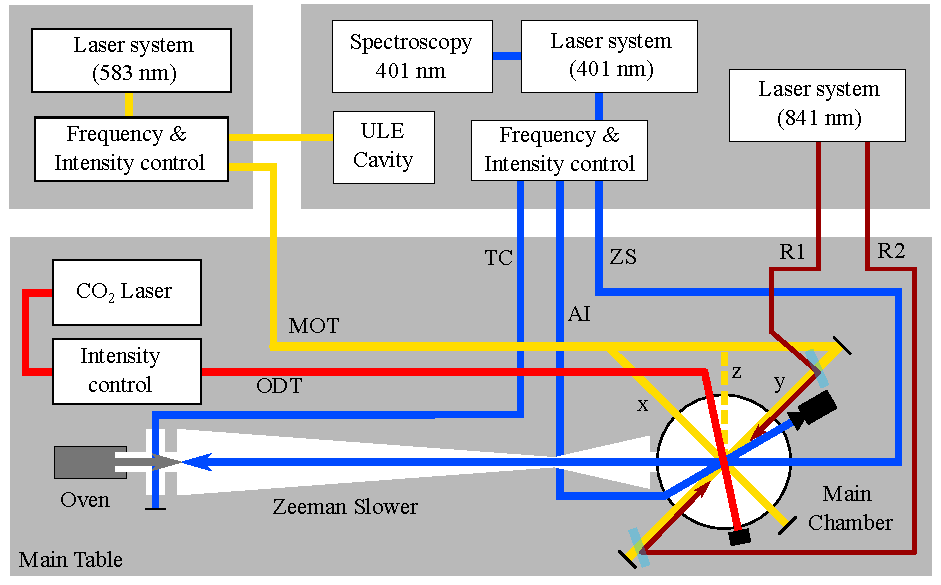
\includegraphics[width=1.\columnwidth]{table_set_up.pdf}
	\caption[Scheme of the experimental setup]{Scheme of the experimental setup. It is divided in three optical tables represented by gray areas. The 401nm laser system is used for the \acf{tc}, \acf{zs} and \acf{ai}. It is generated by a frequency doubled diode laser locked to a spectroscopic signal of the 401nm transition of $^{\text{168}}\text{Er}$. The 583nm laser system is used for the \acf{mot} and is frequency looked to an \acf{ule}. This trap uses 401nm laser beam in three spacial dimensions x, y and z. The $\text{CO}_{2}$ laser is used as main source of an \acf{odt}. The 841nm laser system is used to form the two lattice beams used for the Bragg scattering process which will be described in next Chapter.}\label{fig:table_set_up}. 
\end{figure}

Most of the laser systems in this experiment produce resonant light for the $^{\text{168}}\text{Er}$ atomic transitions. For this reason, these light sources are kept on different optical tables separated from the \ac{uhv} system. Thus, unwanted atom-light interaction that could damage the cooling capabilities of the experiment is reduced. This laser light is guided into the main table by using optical fibers that can be blocked and unblocked through the use of \acp{aom} before the fiber coupler. Allowing for a fast response time (typically a few microseconds) and better control of the experimental phases.

The different phases required to obtain an erbium \ac{bec} are chronologically very organized. There is almost no temporal overlay between phases. This allows for a very accurate description of the experiment by just explaining every procedure in a chronological order. In every cycle, the atoms start in the oven and pass through the \ac{tc} and \acf{zs} to reach the main chamber, where the \ac{mot}, \ac{odt} and evaporative cooling take place to generate the erbium \acl*{bec}.

\subsection{Oven}\label{subsec:oven}

The required first step to form an erbium \ac{bec} consist in transforming a solid state metal, with a high purity of erbium atoms (typically over 99\%), into an atomic beam. There are multiple reasons to why this is necessary. The main one being that it reduces the interaction between atoms and allows for laser cooling and trapping techniques. This will become more clear in the next experimental phases.

In order to produce an erbium beam, an oven of the type known as \Acf{dfc}\footnote{Model DFC-40-10-WK-2B by CreaTec Fischer \& Co. GmbH} is used, operating inside an \ac{uhv} chamber. The left side of Figure \ref{fig:experiment_scheme_1} shows a basic scheme of this device, which is divided into two tantalum wired cavities. The first one is called \Acf{ec} and contains the bulk metal of erbium, which is heated up to \SI{1200}{\degreeCelsius} and sublimated into gas. After this, the erbium gas is transferred through a \SI{3}{\centi\meter} pinhole into the second cavity of the \ac{dfc} known as \Acf{hl}. This last part of the oven is heated a \SI{100}{\degreeCelsius} higher than the \ac{ec} temperature to avoid condensation of material at the pinholes. Lastly, the erbium gas leaves the oven forming an atomic beam through a second pinhole that connects the \ac{hl} cavity with all the following experimental stages. In order to avoid the atomic beam from altering some of these sensitive experimental phases, the second pinhole is closed by a mechanical shutter at these moments. 

The speed at which the atoms are leaving the oven can be estimated in average with a parameter called \ac{rms} velocity $\bar{v}_{RMS}$. For the case of an ideal gas it has been obtained as \cite{Hansch1975}

\begin{equation}\label{eq:rms_velocity}
	\bar{v}_{RMS} = \sqrt{\frac{3 k_B T}{M}}
\end{equation}

This means that for a \ac{hl} temperature of \SI{1400}{\kelvin} the resulting \ac{rms} velocity of the erbium beam leaving the oven is approximately \SI{457}{\meter\per\second}.



\begin{figure}[!htbp]\centering
	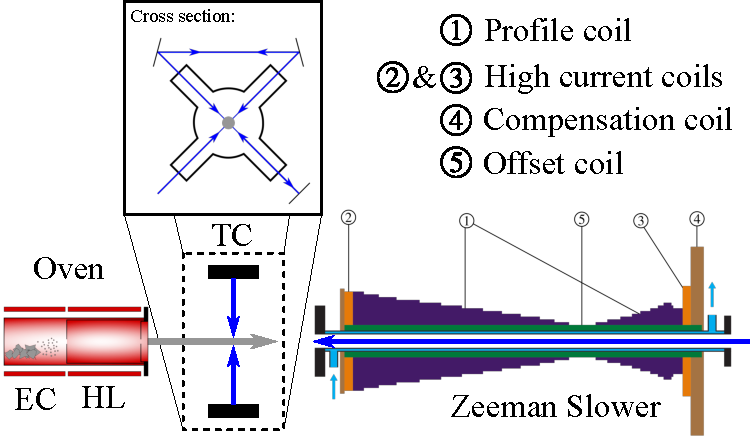
\includegraphics[width=1.\columnwidth]{experiment_scheme_1.pdf}
	\caption[Oven, \acl{tc} and \acl{zs} schemes]{Scheme of the oven, \acl{tc} and \acl{zs}. The atomic beam of erbium and the \SI{401}{\nano\meter} laser beam are represented by gray and blue arrows respectively. A cross section of the \acl{tc} can be seen inside a box. And the different coils used for the \acl{zs} are also represented.}\label{fig:experiment_scheme_1}
\end{figure}



\subsection{Transversal and Optical cooling}

An atomic beam produced by the \ac{dfc} oven presents two main problems: a poor collimation of the beam and a high speed of the erbium atoms forming the beam. These obstacles must be fixed before being able to trap the atoms into an atomic ensemble and form an erbium \ac{bec}. The main purpose of this \Acf{tc} phase is to solve the problem due to poor beam collimation. While the high atomic speed problem will be dealt with in the following \Acl{zs} section. However, these two phases are based in the same underlying physical principle, commonly known as Optical or Laser cooling. 

\subsubsection{Optical cooling}

This technique relies on the force applied on particles by red-detuned near resonant photons. From Equation \eqref{eq:rms_velocity}, it can be seen that the temperature of an ideal gas is proportional to its velocity. So this light-produced force, known as radiation pressure, can be used as a way to lower the temperature of an atomic gas simply by reducing its overall speed. To gain an insight into the physical model of this force, it is necessary to analyse a two-level atomic system  \cite{Metcalf1999}.

Due to this, an two level atom must be considered, which has a ground state $\ket{g}$, an excited state $\ket{e}$ and an energy difference between both states of $\Delta E = \hbar \omega_0$, here $\omega_0$ represents the atomic resonance frequency. The atom at rest can absorb a photon with resonant frequency $\omega_0$. Thus, transferring its energy $\hbar \omega_0$ and momentum $\vec{p}= \hbar \vec{k}$ to the atom. Where $\vec{k}$ represents the photon wave vector, such as for light with wavelength $\lambda$, the wave number results $|\vec{k}| = 2 \pi / \lambda$. According to which was the initial state of the atom before receiving the photon, it can relax into the ground state by spontaneous or by stimulated emission. The first case is produced when the atom was initially at the state $\ket{e}$, which makes the incoming photon trigger an relaxation into $\ket{g}$ of the atom. Resulting in the production of a second identical photon with the same frequency and direction than the triggering one. Because of this, the momentum transfer of the initial photon gets cancelled by the second one and therefore the effective momentum transferred to the atom adds up to zero. However, the second case of spontaneous emission results in a non-zero momentum transfer. Because in this case, the atom is initially in the ground state, allowing it to absorb the initial photon to get in the excited state. After a decay time $\tau$ the atom decays back to $\ket{g}$ and re-emits a second photon in a random direction. Due to the fact, that this photon is at average emitted isotropically in all directions, the momentum transfer produced by the second photon adds up to zero. Resulting in an effective momentum transfer of the atom equal to the initial momentum of the first photon.

In order to obtain an analytical analysis, the Bloch equations must be solved for a two level system. Resulting in the stationary solution for an occupation probability of the excited given by

\begin{equation}\label{eq:probablility_excited_state}
	\rho_{ee} = \frac{s_0/2}{1 + s_0 + \Big(\frac{2\delta}{\gamma}\Big)^2}
\end{equation}

Where $\gamma = 1/\tau$ is the decay rate, $\delta = \omega - \omega_0$ the detuning between laser light and atomic resonance  frequency and $s_0 = I / I_s$ the saturation parameter defined as the ratio of laser light intensity $I$ and saturation intensity $I_s = 2 \pi^2 \hbar c/ 3 \lambda^2 \tau$, with $\lambda$ the light wavelength and $c$ the speed of light. The radiation pressure force can be calculated using Equation  \eqref{eq:probablility_excited_state} as

\begin{equation}\label{eq:radiation_pressure_no_doppler}
	\vec{F} = \hbar \vec{k} \gamma \rho_{ee} = \hbar \vec{k} \gamma \frac{s_0/2}{1 + s_0 + \Big(\frac{2\delta}{\gamma}\Big)^2}
\end{equation}

However, this equation is only valid for a system of coordinates at rest with respect to the atom. This means that for an atom moving at a velocity $\vec{v}$, the light frequency received by the atom will be Doppler shifted an amount  $\Delta \omega_D = -\vec{k}\vec{v}$. By adapting Equation \eqref{eq:radiation_pressure_no_doppler} to the Doppler shift results

 \begin{equation}\label{eq:radiation_pressure}
 	\vec{F} = \frac{\hbar \vec{k} \gamma}{2} \frac{s_0}{1 + s_0 + \Big(\frac{2(\delta-\vec{k}\vec{v})}{\gamma}\Big)^2}
 \end{equation}

This equation for the radiation pressure suggests that a beam of atoms can be slowed down by a red-detuned ($\delta < 0$) counter-propagating optical beam. And therefore, the atomic beam temperature can decreases by following Equation \eqref{eq:rms_velocity}. However, this cooling process presents some limitations because of the spontaneous emission of the second photon. As already said, this spontaneous emission process has a vanishing momentum transfer. But its mean squared value does not vanish, thus heating up the atoms. For a limiting case in which this heating effect equals the optical cooling, an equilibrium temperature is reached known as Doppler limit or Doppler temperature, $T_D$.

\begin{equation}\label{eq:Doppler_limit}
	T_D = \frac{\hbar \gamma}{2 k_B}
\end{equation}

Which is a theoretical temperature limit for an ideal two levels atom \cite{Metcalf1999}. It can be seen from Equations \eqref{eq:radiation_pressure} and \eqref{eq:Doppler_limit}, that there must be a trade off in the experimental value for decay rate of the excited level $\gamma$. In order to achieve a strong enough value for the radiation pressure at the same time that a low enough Doppler temperature. There is however, the capability of cooling down further than the Doppler limit with the use of more refined techniques for multilevel atoms, such as the polarization gradient cooling approach \cite{Dalibard1989}. Nonetheless, for the case of complex multilevel elements like erbium, excited atoms may decay into intermediate states. This limits the cooling process and can suppress it almost completely, due to possible selection rules or high decay times in these intermediate states. If this is our case, the problematic state is commonly called Dark state. To solve this issue, additional pumping lasers or effectively closed transitions must be considered.

\subsubsection{Transversal cooling}

Through the use of Optical cooling physical principles this experimental phase is used to collimate the atomic beam produced by the \ac{dfc} oven. In Figure \ref{fig:experiment_scheme_1}, a scheme and cross section of the \ac{tc} can be seen. The main objective is to increase the flux of atoms passing from \ac{dfc} to the initial part of the \ac{zs} aperture. To achieve this, a crossed optical beam of the red-detuned \SI{401}{\nano\meter} transition, transversal to the atomic beam, is used. As seen in the cross section scheme, the optical cross beam is overlaid with an ingoing and outgoing part. This results in four optical beams traversing the atomic beam in four perpendicular directions. This scheme together with the optical force described Equation \ref{eq:radiation_pressure} leads to radiation pressure acting towards the atomic beam centre, collimating it. Moreover, the high value for the decay rate of $\gamma = \SI{2.22e8}{\per\second}$ for the \SI{401}{\nano\meter} transition (see Table \ref{tab:Transitions}) makes the radiation pressure force considerably strong. In order to enhance the interaction between atomic and light beam, this last one has its shape widened elliptically with the mayor axis parallel to the atomic beam.


\subsection{\Acl{zs}}

As it has already been discussed in the previous section, the second problem that arises is the high speed at which the atomic beam is travelling. At the end of Section \ref{subsec:oven}, a calculation of the average speed of atoms leaving the oven resulted in approximately \SI{457}{\meter\per\second}. However, it has been estimated that the maximal trapping velocity is a few meters per second, for the specific \acl{mot} used in this experiment \cite{Ulitzsch2016}. The main objective of this experimental phase is to reduce the average atomic speed so that it is feasible to trap the atoms in an atomic ensemble. This requires another red-detuned laser beam from the \SI{401}{\nano\meter} transition moving in the opposite direction of the atomic beam. A counter-propagating optical beam transmits radiative pressure to the atomic beam as seen in Equation \eqref{eq:radiation_pressure}. However, as the atomic beam begins to be slowed down, the average velocity of the atoms $\vec{v}$ is reduced and the Doppler shift value $\Delta \omega_D = -\vec{k}\vec{v}$ in Equation \eqref{eq:radiation_pressure} also decreases. This results in a change of the resonance condition and suppression of the radiative pressure, which reduces the slowing effect of the atomic beam. In order to avoid this, the inner splinting of the atomic energy levels must be changed with the use of an spatially varying magnetic field. Thus, at the same time that the beam is being slowed down, the effective atomic resonance is being changed to match a reduction of the Doppler shift $\Delta \omega_D$. The atomic energy shift is affected by the position-dependent magnetic field $\vec{B}$, where the dominant effect is called Zeeman splitting $\Delta \omega_Z$, given by \cite{Zeeman1897}

\begin{equation}
	\Delta \omega_Z = \frac{\mu_{\text{eff}}}{\hbar} |\vec{B}|
\end{equation}

Where $\mu_{\text{eff}}$ represents the effective magnetic moment \cite{Metcalf1999}. By considering the desired case in which the Zeeman and Doppler shifts compensate each other $\omega_Z = -\omega_D$, and using also some basic kinematic theory. The required magnetic field can be obtained as a function of position $z$ at the axis in which the atomic beam is moving:

\begin{equation}\label{eq:magnetic_field_zeeman_slower}
	|\vec{B}(z)| = \frac{\hbar k}{\mu_{\text{eff}}}\sqrt{v_0^2 + 2 a(z-z_0)}
\end{equation}

With $a$ being the deceleration parameter, $v_0$ the maximal velocity at which the atoms can be slowed down and $z_0$ the spacial point where the atom deceleration begins. These types of magnetic fields can be shaped using coils with a spatial dependent number of wires, which is the case for a common \acf{zs} like the one used in this experiment. Figure \ref{fig:experiment_scheme_1} shows a scheme of the \ac{zs} with a counter propagating beam of \SI{401}{\nano\meter} transition providing the radiation pressure to the atomic beam and a group of five independent coils providing the magnetic field described by Equation \eqref{eq:magnetic_field_zeeman_slower}. For more details on the \ac{zs} experimental set-up and the description of these coils refer to \cite{Rehberger2013}.

\subsection{\Acf{mot}}

Once the atomic beam has passed the \ac{zs} and has been slowed down to a few meters per second, the erbium atoms enter the main \ac{uhv} chamber shown in Figure \ref{fig:main_chamber}. The next step requires trapping the atoms in a local region of the main chamber with the use of a \Acf{mot}. Thus, the atomic beam forms an ensemble of atoms with an even lower average velocity, which means a reduction in the erbium atoms temperature within the ensemble. In this case, the \ac{mot} used consists of three pairs of counter-propagating laser beams red-detuned to the \SI{583}{\nano\meter} transition. Each of these beam pairs is perpendicular to the other two, forming three spatial axes inside the main chamber ($x$, $y$ and $z$) with an overlay region where the atomic ensemble will be made. In addition to this, two water cooled coils in an anti-Helmholtz configuration are required to create a quadrupole magnetic field, which is zero inside the overlaying region of the six laser beams. The result of this magneto-optical set up is the generation of a three dimensional spatially dependent restoring force, which binds the erbium atoms to remain inside the overlaying region. To have a physical interpretation of why this is happening, it is necessary to consider a two level atom located inside this region. The atom has a ground state $g$ with a total angular momentum quantum number of $J=0$ and an excited state $e$ with $J'=1$. Due to spatial symmetry and to simplify things even further, just effects in the $z$ axis will be considered. A scheme of this model can be observed in Figure \ref{fig:MOT_Energy}. Because of Zeeman splitting, the magnetic field $B_z = A z$ produced by the anti-Helmholtz coils at the $z$ direction, splits up the atomic states' degeneracies. Thus, for the ground state $m_g = 0$ because $J=0$ and there is no splitting, but for the excited state $m_e = [-1, 0, 1]$ because $J'=1$ splitting this state into three. The resulting force $\vec{F} = F \vec{e_z}$ being applied to an atom at a position $z'$ and a speed $\vec{v} = v \vec{e_z}$ comes from Equation \eqref{eq:radiation_pressure} applied in the two axial directions:

\begin{equation}\label{eq:MOT_force}
	\vec{F} = \frac{\hbar \vec{k} \gamma}{2} \frac{s_0}{1 + s_0 + \Big(\frac{2\delta_+}{\gamma}\Big)^2} - \frac{\hbar \vec{k} \gamma}{2} \frac{s_0}{1 + s_0 + \Big(\frac{2\delta_-}{\gamma}\Big)^2}
\end{equation}

Where:

\begin{equation}\label{eq:delta_plus_minus}
	\delta_\pm = \delta \mp \vec{k} \vec{v} \pm \frac{ \mu_{ \text{eff} } B_{z'} }{ \hbar }
\end{equation}

\begin{equation}\label{eq:mu_eff}
	\mu_{ \text{eff} } = \mu_B (g_e m_e - g_g m_g)
\end{equation}

With $\mu_B$ the Bohr magneton, $g_{g/e}$ the Landé factor and $\pm \vec{k} = \pm |k| \vec{e_z}$ the wave vector of both beams. As a result of this, the atom located in $z'$ will interact most likely with the light beam for which the detuning $\delta_+$ or $\delta_-$ is smaller. This means that an atom moving in any direction away from the \ac{mot} will absorb only photons from the optical beams that can push it towards the \ac{mot}'s centre. Because of the fact that erbium's \SI{583}{\nano\meter} transition has a narrow line-width of \SI{185.71}{\kilo\hertz} (see Table \ref{tab:Transitions}), the type of \ac{mot} used here is commonly known as a narrow-line \ac{mot}, which allows to achieve lower temperatures due to Equation \eqref{eq:Doppler_limit}. The experimental phase of the \ac{mot} can be divided into two main parts. The first one being known as the Loading phase, where the erbium atoms are collected from the \ac{zs}. And lastly, the Compressing phase, where the ensemble of atoms inside the \ac{mot} is compressed by detuning the lasers and magnetic fields. The result of this is a denser and more confined atomic cloud, which is useful for the \ac{odt} phase. Some typical temperatures achieved for erbium clouds trapped in the used \ac{mot} are in the \si{\micro\kelvin} regime. For a more in deep description of the underlying principles of \Aclp{mot}, or a characterization of the used set up, refer to \cite{Metcalf1999, Ulitzsch2016, Roell2016}. 

\pagebreak

\begin{figure}[!htbp]\centering
	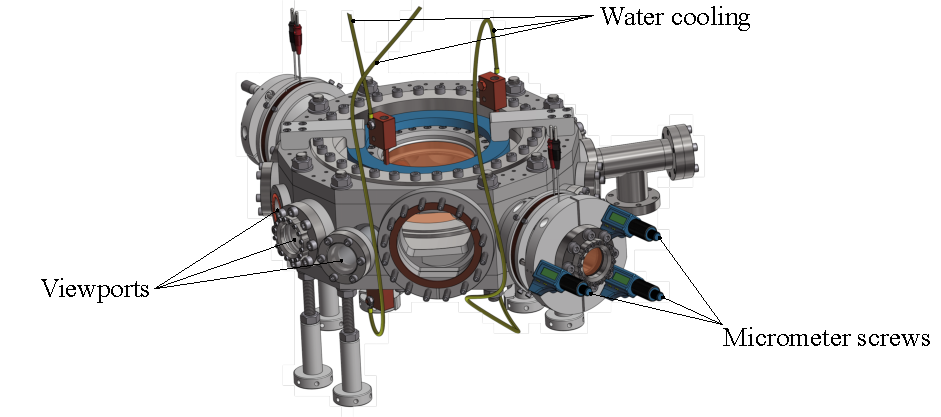
\includegraphics[width=1.\columnwidth]{main_chamber.pdf}
	\caption[Technical drawing of the main chamber]{Technical drawing of the main chamber. It has 17 viewports with different diameters and each one with anti-reflection coatings for the used laser transitions. The chamber also counts with a configuration of water cooled coils inside it, and some micrometer screws connected to lenses for collimation of the different laser beams passing through the ports. }\label{fig:main_chamber}
\end{figure}


\begin{figure}[!htbp]\centering
	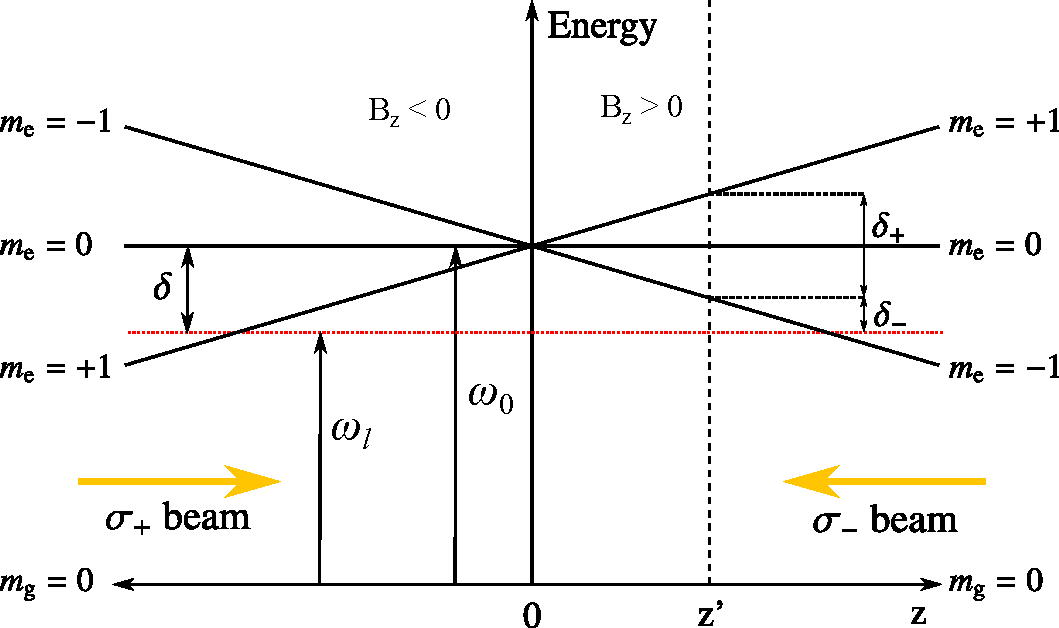
\includegraphics[width=0.9\columnwidth]{MOT_Energy.pdf}
	\caption[Atomic scheme of energies inside the \ac{mot} for a $J=0 \arrowvert J'=1$ transition in the z axis]{Atomic scheme of energies inside the \ac{mot} for a $J=0 \rightarrow J'=1$ transition in the z axis. It shows the Zeeman splinting of the excited state with $J'=1$ into three different states with $m_e = -1, 0, 1$, due to the quadrupole magnetic field produced by two coils in anti-Helmholtz configuration. A counter-propagating pair of circularly polarized laser beams is represented by two yellow arrows. They have a frequency $\omega_l$ illustrated in the energetic scheme by a red dashed line. These optical beams are red-detuned by $\delta = \omega_0 - \omega_l$, where $\omega_0$ is the erbium frequency of the \SI{583}{\nano\meter} transition. Figure modified from original in \cite{Metcalf1999}.}\label{fig:MOT_Energy}
\end{figure}

\subsection{\Acf{odt}}



%%% Local Variables: 
%%% mode: latex
%%% TeX-master: "Thesis"
%%% End: 
% !TEX root = Thesis.tex

%==============================================================================
\chapter{Diffraction of a \acl{bec} with a one-dimensional Optical lattice}
\label{chap:one_dimensional_lattices}
%==============================================================================
In ultracold atoms physics, Optical lattices are defined as periodic standing wave potentials generated by interfering laser beams. Its use allows to replicate results from solid state physics, with the interaction between an ultracold atomic ensemble and an optical lattice being equivalent to the role of electrons in an atomic lattice (i.e. a solid-state crystal) \cite{Lewenstein2007, Bloch2008,Morsch2006}.  However, the use of ultracold systems presents some advantages when comparing with those used in solid state physics. The main one being the capability of changing the optical lattice properties, by simply adjusting parameters like the intensity and detuning of the laser beams forming it. An additional advantage of ultracold atomic systems is the non-existence of crystal defects, which can be a big source of noise in solid states systems \cite{VanDerZiel1978}. This experiment will seek to study how an erbium \ac{bec} behaves when interacting with a one-dimensional optical lattice. In this chapter, an introduction describing the theory behind optical lattices will be shown. After this, it follows a brief description of the implemented set up to form the lattice by using the \SI{841}{\nano\meter} erbium transition (see Table \ref{tab:Transitions}).


\section{Theoretical description of an Optical lattice}

As it can be seen in Figure \ref{fig:lattice_beams}, generating an optical lattice requires the use of two interfering laser beams, with a detuning $\delta$ from the used atomic transition (in this case the \SI{841}{\nano\meter} erbium transition). The main parameter that allows to characterize the experiment is known as the lattice depth $U_0$ and will be determined theoretically in this section by assuming some approximations in the atom behaviour. Moreover, the lattice prosperities can be changed by adjusting the optical intensity of the beams as well as the frequency detuning between beams defined here as $\Delta$. To describe theoretically the interaction of an optical lattice with an atomic ensemble, first is important to characterize accurately the interaction with just one of the optical beams forming the lattice.

\subsection{Dipole interaction of one optical beam}

Taken individually, a laser beam would interact with the atomic cloud like a typical \acf{odt}. Therefore, each beam generates a dipole potential in the atomic ensemble given by Equation \eqref{eq:interaction_potential}. However, in this case there is not a far detuning between the laser beams forming the lattice and erbium atomic transitions. Due to this, assuming the optical fields as quasi-electrostatic does not work any more. But, Equation \eqref{eq:interaction_potential} holds in any case and can be rewritten when the atoms are approximated as a two level scheme following the behaviour of a classical Lorentz oscillator \cite{Grimm2000}. For this case, it can be proved that the complex polarizability $\alpha$ has the form:
\begin{equation}\label{eq:complex_polarizability}
	\alpha = 6 \pi \epsilon_0 c^3 \frac{\Gamma/\omega_0^2}{\omega_0^2 -\omega^2 -i(\omega^3/\omega_0^2)\Gamma} 
\end{equation} 

Where $\omega$ is the optical frequency of the laser beam interacting with the atom ensemble, $\omega_0$ is the atomic transition and $\Gamma$ the on-resonance damping rate. For the classical Lorentz oscillator, this rate is equivalent to $\Gamma = \Gamma_\text{cls}$ where:
\begin{equation}\label{eq:classical_damping_rate}
	\Gamma_\text{cls} = \frac{e^2 \omega_0^2}{6\pi\epsilon_0m_ec^3}
\end{equation}

With $e$ and $m_e$ representing the electron charge and mass respectively. Even though this result is obtained when using the classical Lorentz approximation, an equivalent result can be obtained when considering the semi-classical model of the atom. In which, the atom is considered as a two-level quantum system that interacts with a classical field of light. For the semi-classical model, Equation \eqref{eq:complex_polarizability} is still valid, except for the damping rate $\Gamma$. Now, it corresponds to the spontaneous decay rate of the excited level $\Gamma_\text{smcls} \equiv \gamma$ and is given by
\begin{equation}\label{eq:semiclassical_damping_rate}
	\Gamma_\text{smcls} = \frac{\omega_0^3}{3\pi\epsilon_0 \hbar c^3} \mathopen|\bra{e}\mu\ket{g}\mathclose|^2
\end{equation}

Where $\bra{e}\mu\ket{g}$ stands for the dipole matrix element between ground and excited state. By using Equations \eqref{eq:interaction_potential} and \eqref{eq:complex_polarizability}, for the case of large enough detuning $\delta$ ( making the scattering rate much smaller than $\Gamma$) and low enough intensities $I(\vec{r})$ (avoiding saturation of the excited state), the dipole potential $U_{\text{dip}}(\vec{r})$ can be obtained as
\begin{equation}
	U_{\text{dip}}(\vec{r}) = -\frac{3\pi c^2}{2\omega_0^3} \bigg(\frac{\Gamma}{\omega_0-\omega} + \frac{\Gamma}{\omega_0+\omega}\bigg) \cdot I(\vec{r})
\end{equation} 

Being this equation valid for both the classical and semi-classical model. For most cases, the rotating wave approximation can be applied here because usually the detuning $\mathopen|\delta\mathclose| << \omega_0$. Using this approximation, the dipole potential for one laser beam interacting with an neutral atomic ensemble can be obtained as
\begin{equation}\label{eq:relation_potential_intensity}
	U_{\text{dip}}(\vec{r}) = \frac{3\pi c^2 \Gamma}{2\omega_0^3 \delta} \cdot I(\vec{r})
\end{equation} 

And by assuming the beam to be a Gaussian beam, Equations \eqref{eq:intensity_gaussian} and \eqref{eq:relation_potential_intensity} lead to the exponential behaviour already described in Equation \eqref{eq:dipole_potential}.

\pagebreak

\subsection{One-dimensional optical lattice}\label{subsec:One_dim_optical_lattice}

After considering only the interaction with just one beam, the optical lattice potential $U_\text{lat}(\vec{r})$, generated by two optical beams, has the same relation with the lattice intensity $I_\text{lat}(\vec{r})$ than the previous case described in Equation \eqref{eq:relation_potential_intensity}. Therefore, it can be assumed similarly that:
\begin{equation}\label{eq:relation_lattice_potential_intensity}
	U_{\text{lat}}(\vec{r}) = \frac{3\pi c^2 \Gamma}{2\omega_0^3 \delta} \cdot I_{\text{lat}}(\vec{r})
\end{equation} 

Where $I_\text{lat}(\vec{r})$ is equal to the squared absolute value of the summed electric fields $\vec{E}_1(\vec{r}, t)$ and $\vec{E}_2(\vec{r}, t)$ generated by the two beams. 
\begin{equation}\label{eq:relation_lattice_inesity_fields}
	I_{\text{lat}}(\vec{r}) = \mathopen\big|\vec{E}_1(\vec{r}, t)+\vec{E}_2(\vec{r}, t)\mathclose\big|^2
\end{equation}

This way, assuming that both beams are linearly polarized in the arbitrary $\hat{e}_z$ direction, have the same frequency $\omega$ and are forming a perfectly parallel overlay through the $x$ axis. The electric fields have the expression:
\begin{equation}\label{eq:relation_electric_fields}
	\vec{E}_{1/2}(\vec{r}, t) = \hat{e}_z \sqrt{I_{1/2}(\vec{r})}\cdot e^{-i(\omega t \pm kx)}
\end{equation}

With $I_{1/2}(\vec{r})$ the individual intensity of the laser beams at the point in space $\vec{r}$ from the beam propagation axis. For intensities of the same order $I_{1}(\vec{r}) \sim I_{2}(\vec{r})$, the lattice intensity can be approximated as
\begin{equation}\label{eq:relation_lattice_inesity}
	I_{\text{lat}}(\vec{r}) = 4\sqrt{I_{1}(\vec{r})I_{2}(\vec{r})} \cdot \text{cos}^2(kx)
\end{equation}

Therefore, a final expression for the lattice potential can be obtained when combining Equations \eqref{eq:relation_lattice_potential_intensity} and \eqref{eq:relation_lattice_inesity}. The result is as expected, a temporally static potential with periodicity along the overlaying $x$ axis.
\begin{equation}\label{eq:relation_lattice_potential}
	U_{\text{lat}}(\vec{r}) = U_{0}(\vec{r}) \cdot \text{cos}^2(kx)
\end{equation} 

This important result can be seen in the scheme shown in Figure \ref{fig:lattice_beams}. Where, $U_{0}(\vec{r})$ is known as the lattice depth for which
\begin{equation}\label{eq:relation_lattice_potential_depth}
	U_{0}(\vec{r}) = \frac{6\pi c^2 \Gamma}{\omega_0^3 \delta} \cdot \sqrt{I_{1}(\vec{r})I_{2}(\vec{r})}
\end{equation} 

This is a crucial parameter that allows the complete characterization of the optical lattice. In order to estimate it, $I_{1}(\vec{r})$ and $I_{2}(\vec{r})$ must be considered as Gaussian beam intensities governed by Equation \eqref{eq:intensity_gaussian}. However, in a real experiment for an atomic \ac{bec} localized in a given point in space $\vec{r}$, the alignment between optical beams is never perfect. This means that factors like spacial differences in the propagation axes or different waist sizes between beams, affect very strongly on the effective values of the intensities in Equation \eqref{eq:relation_lattice_potential_depth}. Due to this, two coordinate systems must be considered to account for the atomic ensemble position relative to the first and second beams. This way, the \ac{bec} is located at position $\vec{r}_1$ ($\vec{r}_2$) with respect to beam 1 (beam 2), which has a waist size of $w_1$ ($w_2$) at the atomic ensemble position. Using this argument together with Equations \eqref{eq:intensity_gaussian} and \eqref{eq:relation_lattice_potential_depth}, one gets the final expression for the lattice depth as $U_{0}(\vec{r})=U_{0}(r_1,r_2)$ with
\begin{equation}\label{eq:relation_lattice_potential_depth_final}
	U_{0}(r_1,r_2) = \frac{12 c^2 \Gamma\sqrt{P_1 P_2}}{\omega_0^3 \delta w_1 w_2} \cdot e^{-r_1^2/w_1^2} e^{-r_2^2/w_2^2}
\end{equation} 

In this expression there are two terms that must be accounted for. The first one corresponds to the fraction, with all terms being experimentally measurable within a reasonable uncertainty value. The second one nonetheless, is formed by two exponentials depending on the beams alignment with respect to the atomic \ac{bec} position. Due to this, it is not an easy term to measure because of the big changes that small variation in the position may cause. Therefore, a direct calculation of the lattice depth with the experimental parameters is not feasible and more advanced methods must be considered \cite{Kadau2011}.

\begin{figure}[!htbp]\centering
	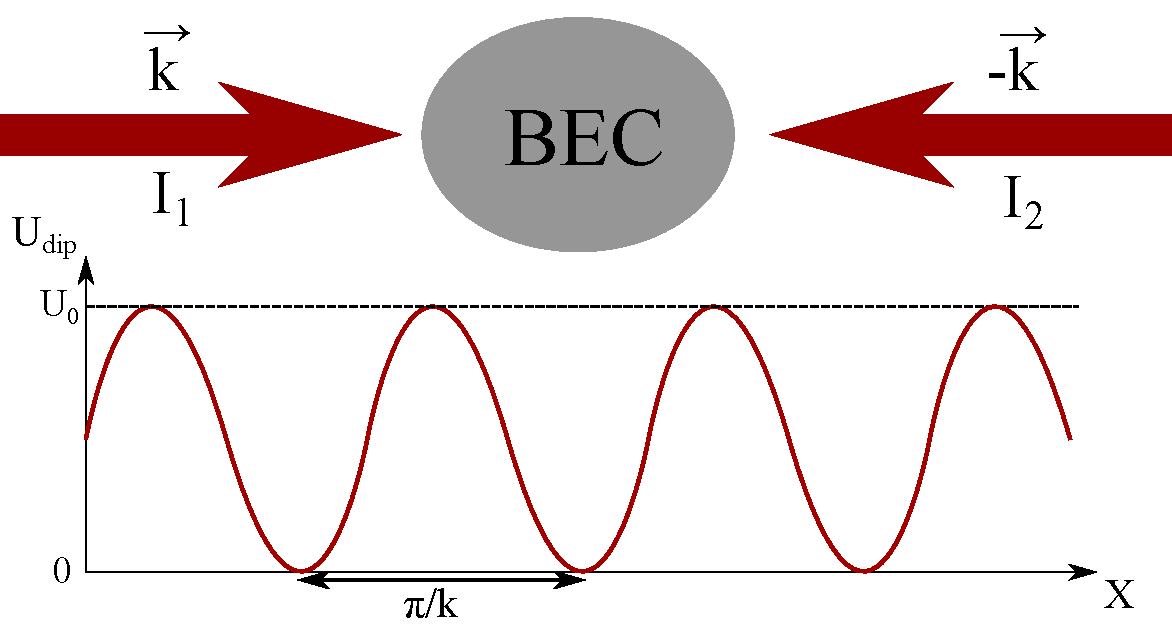
\includegraphics[width=0.7\columnwidth]{lattice_beams.pdf}
	\caption[Scheme of an atomic \ac{bec} interacting with a one dimensional optical lattice]{Scheme of an atomic \ac{bec} interacting with a one dimensional optical lattice. For this case, it has been decided that the optical lattice is generated by two counter-propagating laser beams with wave number $k$, detuned a certain value $\delta$ from the erbium \SI{841}{\nano\meter} transition. Most of the lattice characteristics can be tuned by simply adjusting the beam intensities $I_1$ and $I_2$.}\label{fig:lattice_beams}
\end{figure}

\subsubsection{Moving optical lattice}

Once the lattice potential were obtained for two beams with the same frequency, there is a relevant case of study for which this appreciation is not valid. This is the situation in which there is a small detuning $\Delta$ between both beams. In this case, an additional temporal phase is added to one of the electric fields in Equation \eqref{eq:relation_electric_fields}. This means that the temporally independent expression for the lattice potential of Equation \eqref{eq:relation_lattice_potential}, becomes temporally dependent with the form
\begin{equation}\label{eq:relation_moving_lattice_potential}
	U_{\text{lat}}(\vec{r},t) = U_{0}(\vec{r}) \cdot \text{cos}^2\bigg(kx-\frac{\Delta}{2}t\bigg)
\end{equation} 

Where the intensities have also been assumed to be of the same order $I_{1}(\vec{r}) \sim I_{2}(\vec{r})$. This way, the lattice becomes a periodic potential, which moves along the beam propagation axis with time. Allowing for a different interaction process with the atomic ensemble, which will be described in the following section.


\section{Diffraction of an ultracold atomic ensemble}\label{sec:diffraction_atomic_ensemble}

When an atomic \ac{bec} interacts with an optical lattice, there are multiple processes that may be involved. Therefore, different regimes will appear, based on the lattice properties and interaction time with an atomic ensemble. The main ones, which will be discussed in this thesis, are related with diffraction processes of the ensemble. These two are commonly known as the Bragg and Raman-Nath regimes, which will be discussed in this section \cite{Mueller2008,Ovchinnikov1999}. To give an idea of how this diffraction effects act over an atomic ensemble, its experimental set-up must be considered analogous to the well-known process of light diffraction. Figure \ref{fig:diffraction} shows this analogy between both processes, generating different orders (0th, $\pm$1st ...) as a result. All these orders must fulfil a theoretical restriction known as the Bragg condition, which was initially theorized only for light diffraction by a crystal lattice \cite{Bragg1913}. However, this condition is also valid for atomic diffraction, with the detuning $\Delta$ between optical lattice beams, acting as the restricted parameter.


\begin{figure}[!htbp]\centering
	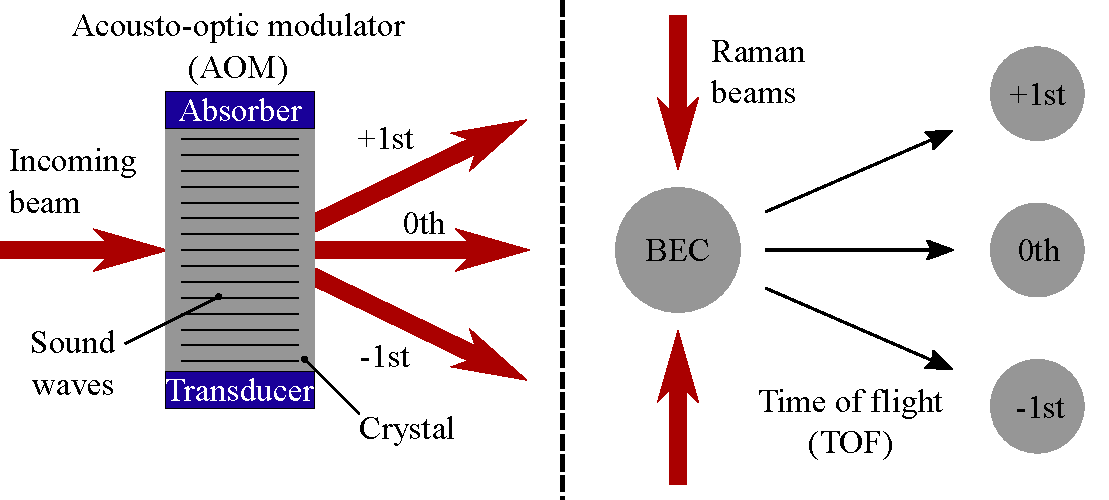
\includegraphics[width=1.\columnwidth]{diffraction.pdf}
	\caption[Analogy between the processes of light diffraction and atomic diffraction of an ultracold ensemble]{Analogy between the processes of light diffraction and atomic diffraction of an ultracold ensemble. The left side shows an light beam being diffracted through the use of an optical device commonly known as an \Acf{aom}. It consists on a solid-state crystal attached to a piezo-electric transducer, which generates sound waves responsible of diffracting the laser beam when it goes through the glass, acting as an optical medium. On the other hand, the right side shows the diffraction process of an atomic \ac{bec} produced by an optical lattice. The ensemble interacts during a certain interaction time $t_{\text{int}}$ with the optical lattice. After a waiting time known as \Acf{tof}, when the ensemble is just falling in vacuum due to gravity, the diffraction process takes place. For both cases, the result generates different orders (0th, $\pm$1st ...), which fulfil the so-called Bragg condition.}\label{fig:diffraction}
\end{figure}


\subsection{Bragg condition}\label{subsec:Bragg_condition}

To give an insight on the process leading to diffraction of an atomic ensemble into the $N$-th order, it is necessary to consider the physical scheme of a 2$N$-photon process. Therefore, the diffraction of an ultracold atomic \ac{bec} can be viewed as a stimulated Raman transition process \cite{Kozuma1999}. Meaning that one can think of the interaction between light and atoms, as photons from one beam being absorbed by the atomic ensemble while the other beam stimulates the emission of photons. This results in a momentum transfer into the ensemble, which is always ``kicked'' an invariant momentum quantity in every of this 2-photon interaction. However, in a 2$N$-photon process, every on this $N$-momentum transfers is produced in the optical lattice axis with a 50$\%$ chance of being in one direction or the other. This explains the appearance of multiple orders in the diffraction process, they are a result of the different 2$N$-photon interactions that the atoms inside an ensemble can produce. Moreover, it also explains why the separation between orders is the same, it is the displacement produced by the momentum transfer resulting from a 2-photon process after a \ac{tof}. This momentum transfer is commonly known as the 2-photon recoil $\vec{P}_\text{rec}$. To illustrate this, an atom must be considered with mass $M$ and initial momentum $\vec{P}_0 = \hbar \vec{k}_0$ along the lattice $x$-axis. The atom interacts with two photons, one coming from the left beam with momentum $\hbar \vec{k}_1$ and other from the right beam with $\hbar \vec{k}_2$. Thus, the total initial momentum of the system before interacting can be expressed as
\begin{equation}
	\vec{P}_\text{i} = \hbar \vec{k}_0 + \hbar (\vec{k}_1 + \vec{k}_2)
\end{equation}

And the total energy before interaction can also be obtained as
\begin{equation}\label{eq:bragg_energy_initial}
	E_\text{i} = \frac{\mathopen\big|\vec{P}_0\mathclose\big|^2}{2M} + \hbar (\omega_1 + \omega_2)
\end{equation}

After interacting, the atom absorbs one of the photons and is stimulated by the other. Resulting in the emission of two identical photons in one of the directions. Arbitrarily, the left photon will considered to be absorbed, hence the right one will be stimulated. The total momentum after interaction results
\begin{equation}
	\vec{P}_\text{f} = \hbar \vec{k}_0 + \hbar (\vec{k}_1 + \vec{k}_2) + 2\hbar\vec{k}_2
\end{equation}

The total energy can be obtained analogously like 
 \begin{equation}\label{eq:bragg_energy_final}
 	E_\text{f} = \frac{\mathopen\big|\vec{P}_0+\vec{P}_\text{rec}\mathclose\big|^2}{2M} + 2\hbar\omega_2
 \end{equation}
 
Where $\vec{P}_\text{rec} = \hbar (\vec{k}_1 + \vec{k}_2)$ represents the 2-photon recoil, the momentum transfer to the atom. It is usually reasonable to consider the case in which both beams forming the lattice have approximately the same wave number $\mathopen\big|\vec{k}_1\mathclose\big| \simeq \mathopen\big|\vec{k}_2\mathclose\big| \equiv k$. Even though, the beam frequencies differ a given value $\Delta$, this parameter is going to be small enough, allowing for the defined approximation. Due to this, an expression for the 2-photon recoil absolute value can be obtained as
\begin{equation}\label{eq:two_photon_recoil}
	\mathopen\big|\vec{P}_\text{rec}\mathclose\big| = 2 \hbar k \text{sin}\bigg(\frac{\theta}{2}\bigg)
\end{equation}

With $\theta$ the angle between wave vectors $\vec{k}_1$ and $\vec{k}_2$, and $k=\frac{2\pi}{\lambda}$ the wave number with wavelength $\lambda$.

By using the energy conservation principle with Equations \eqref{eq:bragg_energy_initial} and \eqref{eq:bragg_energy_final}, the resulting expression gives
\begin{equation}\label{eq:Bragg_condition_1}
	 \Delta_1 = \frac{1}{2M\hbar}\bigg[\mathopen\big|\vec{P}_{\text{rec}}\mathclose\big|^2 + 2\big(\vec{P}_0 \cdot \vec{P}_{\text{rec}}\big)\bigg]
\end{equation}

This gives the value for which the frequency difference between beams $\Delta = \omega_1-\omega_2$, fulfils the so-called Bragg condition in a 2-photon process. Therefore when $\Delta = \pm\Delta_1$, the $\pm1$st diffracted order becomes resonant, meaning that the physical system would tend to diffract more atoms into this order. Due to this, one can conclude that the Bragg condition in this experiment restricts $\Delta$ and therefore the moving lattice speed, which is governed by Equation \eqref{eq:relation_moving_lattice_potential}. The situation can be compared with the light diffraction process described in Figure \ref{fig:diffraction} for an \ac{aom}, with the incidence angle of the incoming beam playing the role of $\Delta$. When this angle fulfils the Bragg condition for the 1st order, it becomes resonant and most of the light will be diffracted through it. 

It can be proved that Equation \eqref{eq:Bragg_condition_1} generalized for a 2$N$-photon has the expression \cite{Kozuma1999}
\begin{equation}\label{eq:Bragg_condition_n}
	\Delta_n = \frac{1}{2M\hbar} \Bigg[n P_{\text{rec}}^2 + \frac{2\big(\vec{P}_0 \cdot \vec{P}_{\text{rec}}\big)}{n}\Bigg]
\end{equation}

Where $n=\pm1, \pm2, \text{...}$ for the different possible diffracted orders. It must be noted that the vectorial product $\vec{P}_0 \cdot \vec{P}_{\text{rec}}$ from Equation \eqref{eq:Bragg_condition_n} becomes zero in average for most of the cases. This is due to the fact that an atomic \ac{bec} can be considered static with respect to the optical lattice during the interaction time $t_{\text{int}}$. Thus, the resonance condition for the different orders can be obtained from Equations \eqref{eq:two_photon_recoil} and \eqref{eq:Bragg_condition_n} as
\begin{equation}\label{eq:Bragg_condition}
	\Delta_n = \frac{2n\hbar k^2}{M}
\end{equation}

For a lattice formed by two counter-propagating waves.

\subsection{Rabi oscillations}\label{subsec:Rabi_oscillations}

As it has already been said, the diffraction of an atomic \ac{bec} with optical lattices can be considered as a 2$N$-photon process. This sort of processes are also known as Raman transitions. The energetic scheme of a 2-photon Raman transition process, like the one discussed in previous section, can be seen in Figure \ref{fig:raman_scheme} \cite{Kozuma1999}. Therefore, the system acts an effective 2-level scheme formed by the initial momentum state $\ket{g, 0}$, together with the final state $\ket{e, 2\hbar k}$ for the 1st diffraction order. This results in Rabi oscillations appearing in the population number of both states, analogously to what happens for the case of a real 2-level system \cite{Foot2005}. Thus, the diffraction of an atomic \ac{bec} produces oscillations in the population rate of the 1st diffracted order as a function of the interaction time $t_\text{int}$ between optical lattice and ensemble \cite{Martin1988}. In order to make calculations easier, the experimental situation will always use an optical lattice with a shaped like squared well in time. This way, the lattice will be on with constant intensity during a time $t_{\text{int}}$ and completely off the rest of experimental phases. For the case of a Raman transition like the one disused in Figure \ref{fig:raman_scheme}, the population in a first resonant ($\Delta=\Delta_1$) diffracted order $\ket{g, 2\hbar k}$ as a function of the interaction time with the lattice can be expressed as
\begin{equation}
	P_1(t_\text{int}) = \text{sin}^2\bigg(\frac{\Omega_\text{eff} t_\text{int}}{2}\bigg)
\end{equation}

Resulting in the well-known Rabi oscillations like in the case of an atomic 2-level system. The variable $\Omega_\text{eff}$ is playing here the role of effective Rabi frequency for the 2-photons Raman transition. It is commonly called 2-photon Rabi frequency and, for the first resonant order, it can be expressed as
\begin{equation}\label{eq:effective_Rabi_frequency}
	\Omega_\text{eff} = \frac{\Omega_1 \cdot \Omega_2}{2\delta}
\end{equation}

\begin{figure}[!htbp]\centering
	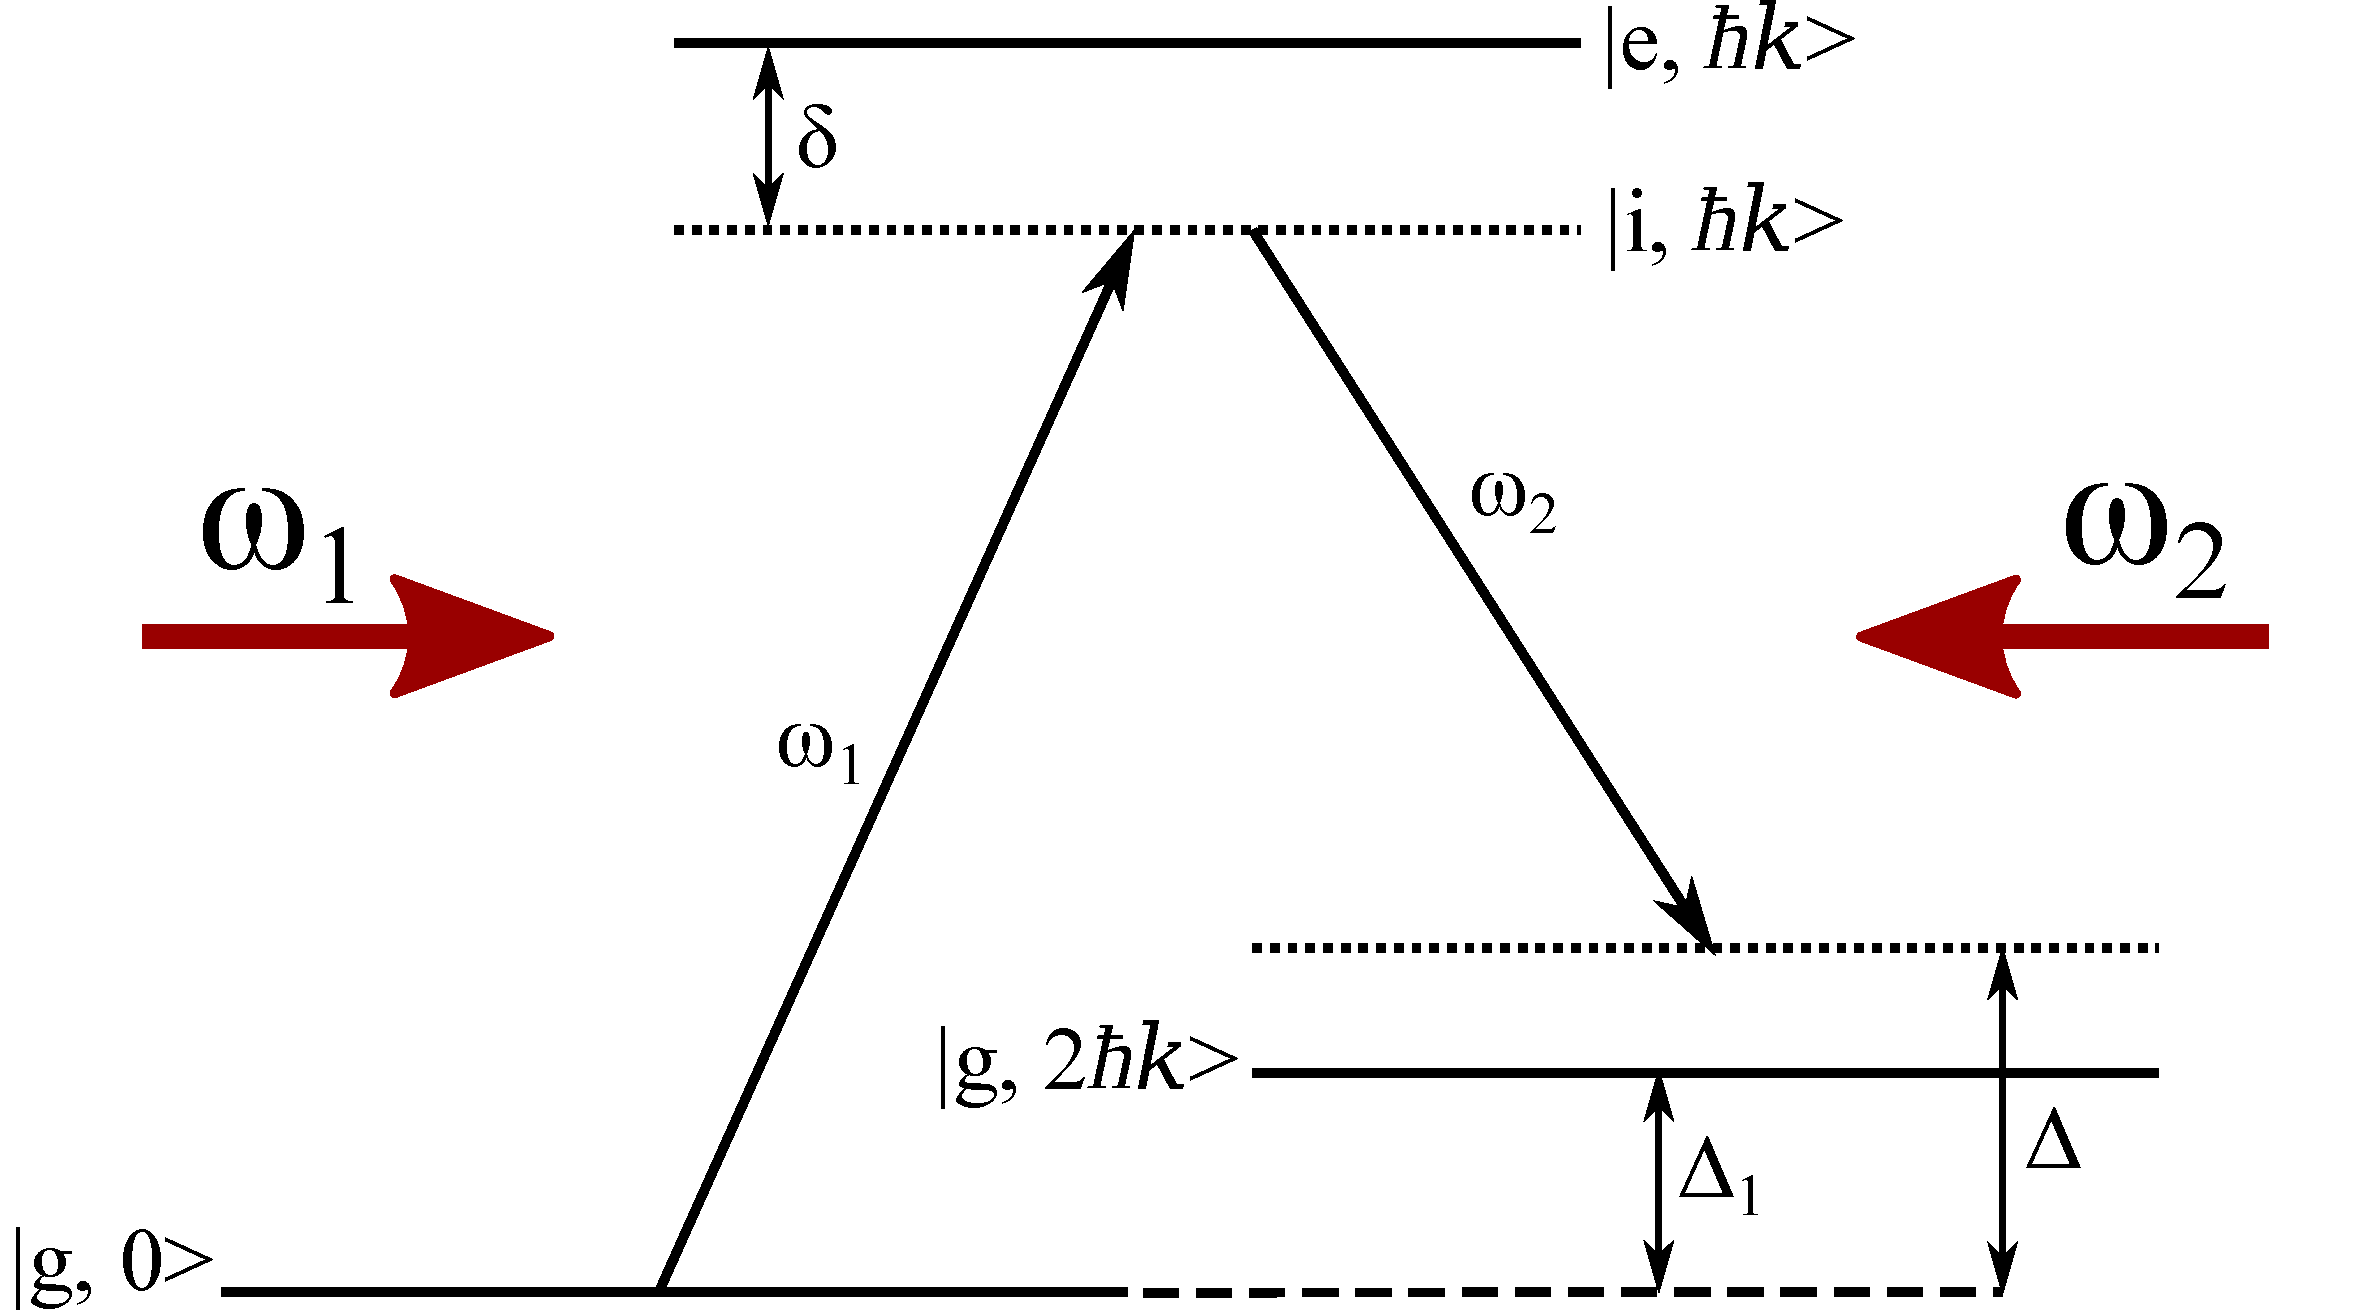
\includegraphics[width=0.8\columnwidth]{raman_scheme.pdf}
	\caption[Energy scheme of the 2-photon Raman transition process]{Energy scheme of the 2-photon Raman transition process. The 2-level atom is initially in the state $\ket{g, 0}$, with $g$ representing the atomic ground state and 0 the null momentum transferred initially to the atom. Then, the atom absorbs a first photon with frequency $\omega_1$, which stimulates it to an imaginary state $\ket{i, \hbar k}$. Finally, the atom emits a second photon with frequency $\omega_2$ through stimulated emission. It must be noted that the momentum transfer has been considered for two counter-propagating photons ($\theta=\pi$ in Equation \eqref{eq:two_photon_recoil}), and also that $\Delta_1$ represents the resonance condition for the first order given by Equation \eqref{eq:Bragg_condition} with $n=1$. Therefore, when $\Delta = \Delta_1$ the condition is fulfilled for this order and the energetic transition gets enhanced. Moreover, to avoid real excitation of the atom into $\ket{e, \hbar k}$, which produces spontaneous emission processes, the detuning from atomic resonance $\delta$ must be large enough. }\label{fig:raman_scheme}
\end{figure}

The variables $\Omega_1$ and $\Omega_2$ represent the single photon Rabi frequency for the atomic 2-level system interacting with a photon from the left and right laser beam respectively \cite{Foot2005}. By using the electric dipole approximation (the wavelength transition can be considered much greater than the typical size of the atom) and considering both beams to be linearly polarized in the $z$ direction, the single photon Rabi frequency can be considered as
\begin{equation}
	\Omega_i = \frac{eZ_{12}}{\hbar} \mathopen|\vec{E}_{i}\mathclose(\vec{r})|
\end{equation} 

Where $e$ is the electron charge, $eZ_{12}=\bra{g}\mu\ket{e}$ the dipole matrix element and $\mathopen|\vec{E}_{i}(\vec{r})\mathclose|$ the electric field amplitude at the point $\vec{r}$ produced by beam $i\in [1,2]$. Therefore, using the relation between electric field amplitude and optical intensity in vacuum is given by
\begin{equation}
	\mathopen|\vec{E}_{i}(\vec{r})\mathclose| = \sqrt{\frac{2}{c \epsilon_0}}\sqrt{I_i(\vec{r})}
\end{equation}

A relation between the 2-photon Rabi frequency and the optical lattice depth can be obtained simply by using the two previous expressions together with Equations \eqref{eq:relation_lattice_potential_depth} and \eqref{eq:effective_Rabi_frequency} as \cite{Ovchinnikov1999}
\begin{equation}
	U_0 = 2\hbar\Omega_\text{eff}
\end{equation}

Where the semi-classical approximation has been used $\Gamma=\Gamma_\text{smcl}$ given by Equation \eqref{eq:semiclassical_damping_rate}. This shows a direct relation between the 2-photons Rabi frequency of the diffraction process and the optical lattice depth. It had been shown that this is an important factor required to characterize the system but it could not be estimated experimentally in an accurate way. Now, it is possible to estimate the optical lattice depth by obtaining just the 2-photon Rabi frequency. It must be noted that the linear factor $2\hbar$ may not hold for some cases, where a really high accuracy must be needed, so multiple alternative calibration methods have been proposed \cite{Ovchinnikov1999,Cabrera2018, Friebel1998,Cristiani2002}. However, the topic is out of reach for this thesis, with a complex calibration of the lattice being a possible pending job for the future. As a side note, the calculations shown here can be generalized for 2$N$-photon processes \cite{Giltner1995}. With the effective Rabi frequency for any resonant $n$ diffracted order being
\begin{equation}\label{eq:effective_Rabi_frequency_n}
	\Omega_\text{eff}^{(n)} = \frac{(\Omega_1 \cdot \Omega_2)^n}{2^{4n-3}((n-1)!)^2\delta^n\omega_r^{n-1}}
\end{equation}

Here, the commonly used  parameter $\omega_r$ is known as recoil frequency and has the expression
\begin{equation}
	\omega_r = \frac{\Delta_1}{4} = \frac{\hbar k^2}{2M}
\end{equation}

Lastly, note that Equation \eqref{eq:effective_Rabi_frequency} can be reached for the first order $n=1$ with Equation \eqref{eq:effective_Rabi_frequency_n}. 

\subsection{Diffraction regimes}

Once the interaction process between an atomic \ac{bec} and optical lattice has been described, one can take a closer look to the system in a more general approach. This way, two different regimes can be distinguished by analysing the Hamiltonian for atoms interacting with an optical lattice as \cite{Mueller2008}
\begin{equation}
	\hat{H}= \frac{\hat{p}^2}{2M} + U_\text{lat}
\end{equation}

Where $U_\text{lat}$ represents the lattice potential described by Equation \eqref{eq:relation_lattice_potential}. Therefore, the resulting Schr\"odinger equation looks like
\begin{equation}\label{eq:Schroedinger}
	i\hbar \dot\psi(x,t) = -\frac{\hbar^2}{2M}\frac{\partial^2 \psi(x,t)}{\partial x^2} + 2\hbar \Omega_\text{eff} \text{cos}^2(kx)\cdot\psi(x,t)
\end{equation}

With $\psi(x,t)$ being the wave function of the 2-level atoms and $\dot\psi(x,t) \equiv \frac{\partial \psi(x,t)}{\partial t}$ the temporal partial derivative. In order to reach this expression, it is required to assume that the atomic detuning is much greater than the excited state linewidth $\Delta \gg \Gamma, \Omega_1, \Omega_2, \omega_r$. This avoids the excitation of most the atoms into its excited state, allowing for $\psi(x,t)$ to be considered the wave function of atoms in the ground state. Moreover, the system have been assumed to be a one dimension problem, with the atoms being only able to interact with the optical lattice in the $x$ direction. As it can be seen, the rest of parameters related with atomic, optical and alignment properties of the system are conveniently hidden within the 2-photon Rabi frequency $\Omega_\text{eff}$. For the case in which $\Omega_\text{eff}$ is not time dependant, Equation \eqref{eq:Schroedinger} enters under the classification group known as Mathieu's differential equations \cite{Mathieu1868}. This type of equation can not generally be solved analytically, which results in the need of simplifying the problem by distinguishing different regimes. This paper will approach the topic by discussing only the two main regimes in a qualitative way. For a more in-depth study, please refer to \cite{Mueller2008, Meystre2001, Ovchinnikov1999, Kadau2011,Keller1999}.

\subsubsection{Raman-Nath regime}
In the case of very short interaction times $t_\text{int}$, the atoms move only by a very small distance compared to the lattice period $\pi/k$. Therefore, the movement of atoms during the lattice pulse can be neglected, which allows to remove the kinetic energy term in Equation \eqref{eq:Schroedinger} (first term on the right hand side). This is known as Raman-Nath approximation and was first introduced in the study of light diffraction with sound waves, acting as a thin grating \cite{Raman1935}. After removing the kinetic energy term, the Schr\"odinger equation becomes solvable. This solution splits the ground sate wave function into multiple $n$ terms with a momentum transfer of $2n\hbar k$, representing the diffraction orders described during this section.
\begin{equation}
	\psi(x,t) = \sum_{n=-\infty}^{+\infty}g_n(t)e^{i 2nkx}
\end{equation}

With the coefficients of every diffraction order given by Bessel functions of the first kind \cite{Mueller2008}
\begin{equation}
	g_n(t) = (-i)^n J_n(\Omega_\text{eff} t)
\end{equation}

Therefore, the resulting population probability of any diffraction order $n$ after an interaction time with the lattice of $t_\text{int}$ can be expressed as
\begin{equation}\label{eq:population_Raman_Nath}
	P_n(t_\text{int}) = J_n^2(\Omega_\text{eff} t_\text{int})
\end{equation}

As a result, multiple diffraction orders are generated in this regime, each one with a population probability given by Equation \eqref{eq:population_Raman_Nath}. From a physical point of view, the diffraction into multiple orders can be understood as a result of the energy uncertainty due to short interaction times. Initially, this number of diffraction orders increases with $t_\text{int}$. However, after a certain limit, the number of orders stops increasing by effect of the kinetic energy term in the Hamiltonian. This can be justified by using the argument of energy-momentum conservation. Due to the dispersion relation being quadratic for atoms and linear for light, which avoids the conservation of energy and momentum for higher orders. This effect can again be compared with the process of phase mismatch appearing in non-linear optics. The saturation of diffraction orders is what restricts the regime, and it can be proved, that the Raman-Nath approximation holds only for interaction times $t_\text{int} \ll 1/\sqrt{2\Omega_\text{eff} \omega_r}$ \cite{Meystre2001}. 

\subsubsection{Bragg regime}
For the case of longer interaction times, the effects of energy-momentum conservation are very strong and do not permit the kinetic energy term removal in Schr\"odinger equation. The kinetic contribution increasingly limits the number of allowed diffraction orders, at the point of permitting only two for a low enough value of the lattice depth. This can be understood because, in very long interaction times, the energy uncertainty stops being a contributing factor. Moreover, the kinetic term dominates, forcing the Bragg condition with the argument of energy-momentum conservation. Due to this, the described case is commonly known as the Bragg scattering regime, because of its similarities with Bragg diffraction of light through a thick grating in optics, as already discussed in this Section. It means that, in order to diffract the atomic ensemble into a given $n$ order, the Bragg condition given by Equation \eqref{eq:Bragg_condition} must be fulfilled. This way, the whole system can be understood as a 2$N$-photon Raman process behaving like an effective 2-level system. Resulting in Rabi oscillations appearing between the $n$ and 0th order for varying interaction times. This means that for the Bragg regime, all the theoretical processes described in Sections \ref{subsec:Bragg_condition} and \ref{subsec:Rabi_oscillations} have a physical correspondence with the system behaviour.

\section{Experimental realization of a one-dimensional optical lattice}

The optical lattice, required to achieve the diffraction processes of an ultracold atomic ensemble, is obtained with the use of two counter-propagating optical beams. The experimental set-up used can be seen in Figure \ref{fig:raman_set_up}. The laser beams used to for the lattice are generated by a titanium-sapphire laser, which is frequency controlled to the erbium \SI{841}{\nano\meter} transition (see Table \ref{tab:Transitions}). In order to have a great control over the interaction time with the atom ensemble, both laser beams are coupled into \acp{aom}. This way, only the first orders of the \acp{aom} are coupled into the fibres R1 and R2, allowing to switch the optical lattice at very fast times on the order of a few hundreds nanoseconds \cite{Helten2019}. The polarization of both beams is being controlled with the use of $\lambda/2$ wave-plates together with \acfp{pbs}. This allows to set the linear polarization axis of both beams in the same axis $z$, which has been a required condition in Sections \ref{subsec:One_dim_optical_lattice} and \ref{subsec:Rabi_oscillations}. For a more in-depth characterization of the experimental set-up described here, refer to \cite{Helten2019}.



\begin{figure}[!htbp]\centering
	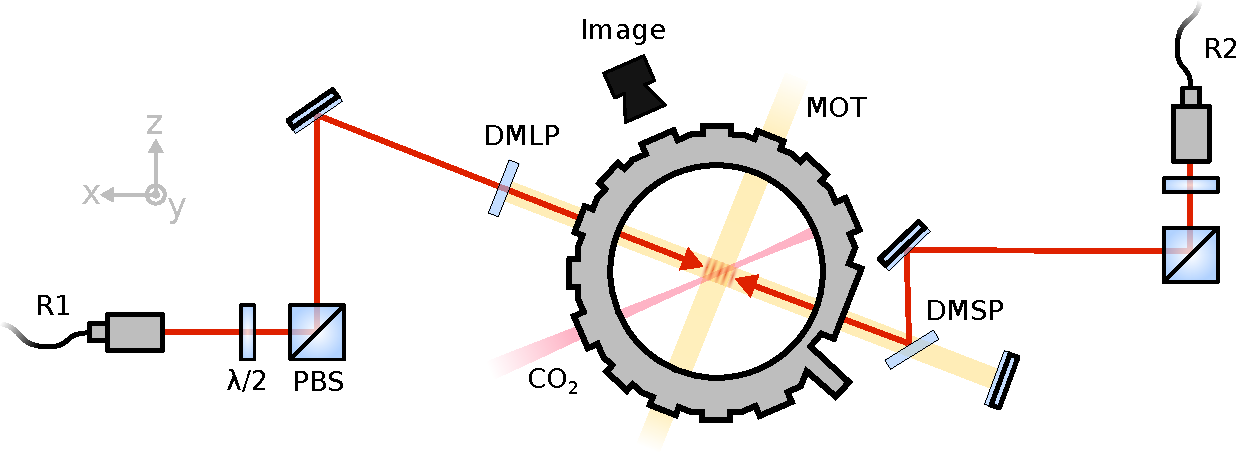
\includegraphics[width=1\columnwidth]{raman_set_up.pdf}
	\caption[Experimental set-up for the optical lattice beam formed inside the \ac{uhv} main chamber]{Experimental set-up for the optical lattice beam formed inside the \ac{uhv} main chamber. The laser beams forming this lattice were detuned a value $\delta$ from the used erbium transition of \SI{841}{\nano\meter}, and are represented by the two counter-propagating red arrows. These beams have been coupled inside the chamber through one of the \ac{mot} axis, by using dicrotic long-pass (DMLP) and short-pass (DMSP) mirrors. Figure taken from \cite{Helten2019}.}\label{fig:raman_set_up}
\end{figure}


%%% Local Variables: 
%%% mode: latex
%%% TeX-master: "Thesis"
%%% End: 

% !TEX root = Thesis.tex

%==============================================================================
\chapter{Towards Raman manipulation of spin-momentum state components}
\label{chap:raman_manipulation}
%==============================================================================

After the theoretical description of the Raman processes occurring in the diffraction of ultracold atomic ensembles, the following step consists in the generation of momentum and spin states components. The process has a strong resemblance with the previously described, with the added factor that now every momentum state also carries a different internal energy state. This is due to Raman transitions taking place inside the Zeeman levels that erbium's ground state was split into. For the experimental process to function as expected, it is required a given magnetic field $\vec{B}_\text{R} = B_{\text{R}} \vec{e}_x$ along the optical lattice axis $x$. This field will produce the Zeeman splitting of the ground state, and the optical lattice will be in charge of producing the Raman transitions, separating the atomic ensemble into multiple energy levels. However, two photon detuning condition must be fulfilled for this process to happen, and now it corresponds with the energy difference between two Zeeman split states $\Delta E_\text{R} = g_J \mu_B B_\text{R}$ \cite{Foot2005}. Due to this, knowing the exact value of $\Delta E_\text{R}$ becomes a key factor, and any background magnetic fields  affecting the \ac{bec} can produce values for the Zeeman splitting very different to the expectation. For this reason, a preparatory experiment must be carried out, that allows the estimation of $\Delta E_\text{R}$ and helps with the compensation of background fields in favour of the known $\vec{B}_\text{R}$ field.

\section{\Acl{rf} transitions and the Stern-Gerlach experiment}

The objective of this experiment is to quantify the Zeeman splitting induced into an erbium \ac{bec}. As it can be seen in Figure \ref{fig:erbium_scheme}, the energetic ground state of erbium has a total electronic angular momentum of $J = 6$. When the atomic ensemble is being affect by a magnetic field $\vec{B}_\text{H}$, the ground state gets Zeeman split into $2J+1 = 13$ energy states with the secondary quantum number $m_J = \text{-6, -5, ..., +6}$, each state with energy \cite{Foot2005}
\begin{equation}
	E_\text{Ze} = g_J \mu_B m_J B_\text{H}
\end{equation}

Where $g_J$ represents the Landé g-factor and for this case it is $g_J\approx11/6$. Due to the way in which the experimental set-up is constructed, the \ac{mot}'s \SI{583}{\nano\meter} beam light that interacts with erbium in the $z$ axis, by pushing the atoms against gravity, is $\sigma^-$ polarized \cite{Ulitzsch2016}. Due to the fact that this beam interacts mostly with the atomic ensemble, it forces the atoms to remain the energetic state with $m_J = -6$. This prevents the direct splitting of the erbium \ac{bec} into different orders by regarding energetic differences. To allow for transitions between these different Zeeman states, the atomic ensemble must interact with a \acf{rf} pulse. Moreover, in order to distinguish which orders the \ac{rf}-pulse has transitioned the atomic ensemble into, a Stern-Gerlach experiment must be performed. This consists in the use of a magnetic inhomogeneous field $B_\text{IH}(\vec{r})$ that separates the atomic \ac{bec} spatially according the quantum number $m_J$. The force that allows this is commonly called Stern-Gerlach force and is due to the non-zero gradient applied to the Zeeman term in the hamiltonian \cite{Foot2005}
\begin{equation}
	\vec{F}_\text{SG}(\vec{r}) = \grad{(\vec{\mu}\cdot\vec{B}_\text{IH}(\vec{r}))}
\end{equation}

Where $\vec{\mu}$ represents the atomic magnetic moment. Therefore, for $B_\text{IH}(\vec{r})$ pointing in any arbitrary $z$ direction, the force applied to the different $2J+1$ levels can be obtained as
\begin{equation}\label{eq:Stern-Gerlach_force}
	\vec{F}_\text{SG}(\vec{r}) = - g_J \mu_B m_J \frac{\partial B_\text{IH}(\vec{r})}{\partial z}
\end{equation}

Which is $m_J$ dependant and produces, as a result, different contributions to the energetic states. This kind of force will make possible the separation of a \ac{bec} in Zeeman orders, and the analysis of internal energetic behaviour after the interaction with a given \ac{rf}-pulse. The use of both these tools permits the creation of an experimental set-up that can quantify the energetic difference between contiguous Zeeman orders
\begin{equation}\label{eq:Zeeman_splitting_difference}
\Delta E_\text{Ze} = g_J \mu_B B_\text{H}
\end{equation}

For a given spatially homogeneous field $\vec{B}_\text{H}$, interacting initially with an atomic ensemble. The experimental procedure can be described as follows:
\begin{itemize}
	\item First, there is a change in the magnetic field $\vec{B}_\text{H}$ acting on the atomic \ac{bec} during its final formation process, the last \SI{10}{\milli\second} of the evaporation cooling phase. This allows to change in different experiment cycles the homogeneous magnetic field $\vec{B}_\text{H}$ and therefore, the Zeeman splitting of the \ac{bec} ground energy level, given by $\Delta E_\text{Ze}$ in Equation \eqref{eq:Zeeman_splitting_difference}.
	\item Then, \SI{2}{\milli\second} after the evaporation phase, the \ac{rf}-pulse is used while $\vec{B}_\text{H}$ is kept unchanged. This \ac{rf}-pulse has a given duration $t_\text{RF}$, an intensity $I_\text{RF}$ and a frequency $\nu_\text{RF}$. As a result, the erbium \ac{bec} transitions between the initial state $m_J=-6$ to the rest of states, when $\nu_\text{RF}\approx\frac{\Delta E_\text{Ze}}{\hbar}$ the resonant frequency for the Zeeman transition. Moreover, due to the fact that these transitions also result in Rabi oscillations, the magnitudes $t_\text{RF}$ and $I_\text{RF}$ must be adjusted to produce $\frac{\pi}{2}$ pulses and favour the atomic transitions into the rest of Zeeman states.
	\item Finally, after the atomic \ac{bec} interaction with the \ac{rf}-pulse, the ensemble falls due to gravity during a \acl{tof} $t_\text{TOF}$. In this time period, the magnetic field gradient $B_\text{IH}(\vec{r})$ is activated and the atomic \ac{bec} receives a state dependant Stern-Gerlach force given by Equation \eqref{eq:Stern-Gerlach_force}. This results in the spacial separation of the Zeeman levels after the \ac{tof}, which can be imaged by the absorption imaging phase.
\end{itemize}

As a result, the experiment allows to measure the resulting orders after a \ac{rf}-\ac{bec} interaction. By varying $\nu_\text{RF}$, one can make a measurement of the resonant frequency to the Zeeman splitting produced by any homogeneous field $\vec{B}_\text{H}$. In addition to the transition's line-width estimation, which is a parameter deeply related to the stability of $\vec{B}_\text{H}$ during the interaction time $t_\text{RF}$. To conclude, the experiment allows to measure the Zeeman splitting of any given field $\vec{B}_\text{H}$, compensate for the effect $\Delta E_\text{Ze}\approx0$ by changing $\vec{B}_\text{H}\rightarrow \vec{B}_\text{Comp}$, and also permits to add any wished field $\vec{B}_\text{H} = \vec{B}_\text{Comp} + B_{\text{R}} \vec{e}_x$ in the desired lattice $x$ direction, which results in $\Delta E_\text{Ze}\approx\Delta E_\text{R}$ the Zeeman splitting between orders in the $x$ axis. Resulting in a fairly good estimation of $\Delta E_\text{R}$ due to $\vec{B_{\text{R}}}$, which will give the two photon detuning condition for Raman manipulation in the following section. This procedure and the experimental set-up have been described in more detail here \cite{Ulitzsch2016}.

\section{Raman manipulation of spin-momentum state components}

\begin{figure}[!htbp]\centering
	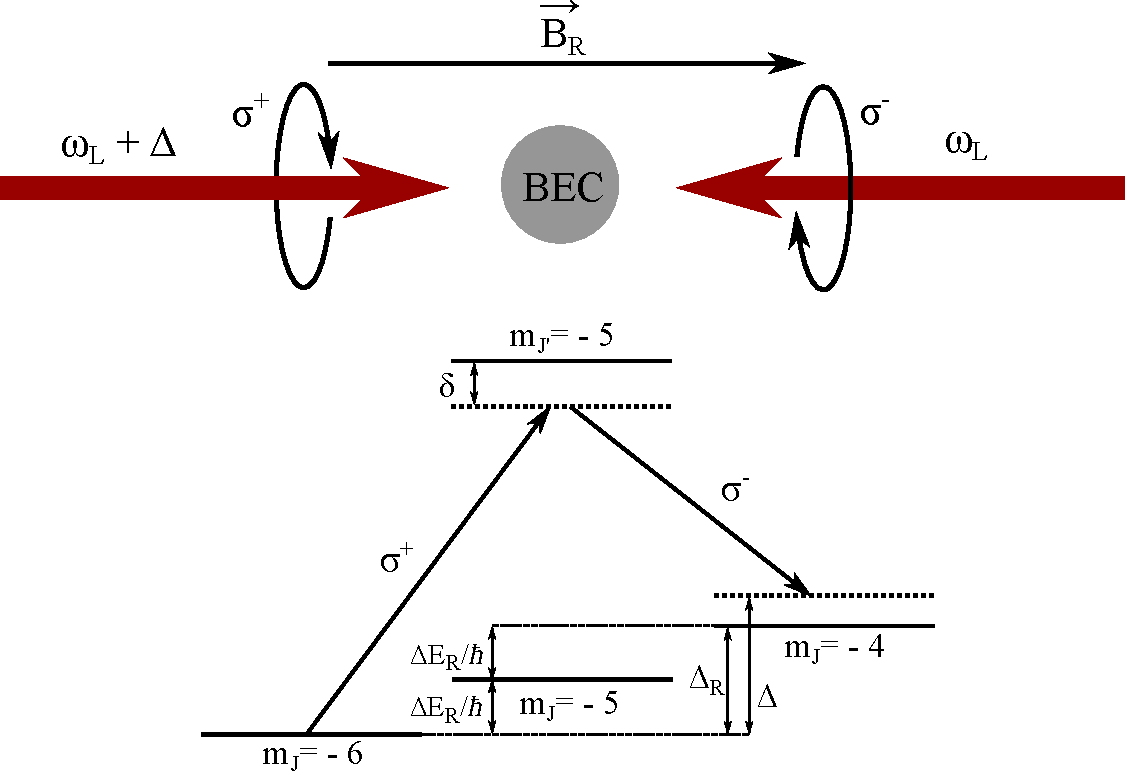
\includegraphics[width=0.8\columnwidth]{rama_spin_mainpulation.pdf}
	\caption[Experimental and energetic scheme of the 2-photon Raman transition process in the spin-momentum configuration]{Experimental and energetic scheme of the 2-photon Raman transition process in the spin-momentum configuration. In this case, the optical scheme is very similar to the described in Chapter \ref{chap:one_dimensional_lattices} with the addition of a magnetic field $\vec{B}_\text{R}$ in the lattice direction $x$ and the circular polarization $\sigma^\pm$ of both beams forming the lattice. Moreover, the energetic scheme also relates to the Raman process described in Chapter \ref{chap:one_dimensional_lattices}, with the only difference that now the two photon detuning condition becomes the so-called Raman condition given by $\Delta_\text{R} \equiv 2\Delta E_\text{R}/\hbar$. As a result, the orders generated in the Raman process not only have different momentum components but also spin values  $m_\text{J}=-6 \rightarrow m_\text{J}=-5$, which means internal energetic changes in the different generated orders. }\label{fig:raman_manipulation}
\end{figure}

%%% Local Variables: 
%%% mode: latex
%%% TeX-master: "Thesis"
%%% End: 

% !TEX root = Thesis.tex

%==============================================================================
\chapter{Results and discussion}
\label{chap:results_and_discussion}
%==============================================================================



%%% Local Variables: 
%%% mode: latex
%%% TeX-master: "Thesis"
%%% End: 

% !TEX root = Thesis.tex

%==============================================================================
\chapter{Conclusion and outlook}
\label{chap:outlook}
%==============================================================================



%%% Local Variables: 
%%% mode: latex
%%% TeX-master: "Thesis"
%%% End: 


% Uncomment the following command to get references per chapter.
% Put it inside the file or change \include to \input if you do not want the references
% on a separate page
% \printbibliography[heading=subbibliography]

%------------------------------------------------------------------------------
% Use biblatex for the bibliography
% Add bibliography to Table of Contents
% Comment out this command if your references are printed for each chapter.
\printbibliography[heading=bibintoc]

%------------------------------------------------------------------------------
% Include the following lines and comment out \printbibliography if
% you use BiBTeX for the bibliography.
% If you use biblatex package the files should be specified in the preamble.
% \KOMAoptions{toc=bibliography}
% {\raggedright
%   \bibliographystyle{../Template/refs/atlasBibStyleWithTitle.bst}
%   % \bibliographystyle{unsrt}
%   \bibliography{./thesis_refs,../Template/refs/standard_refs-bibtex}
% }

%------------------------------------------------------------------------------
\appendix
% \part*{Appendix}
% Add your appendices here - don't forget to also add them to \includeonly above
%%------------------------------------------------------------------------------
\chapter{Useful information}
\label{sec:app}
%------------------------------------------------------------------------------

In the appendix you usually include extra information that should be
documented in your thesis, but not interrupt the flow.

%%% Local Variables: 
%%% mode: latex
%%% TeX-master: "../Thesis"
%%% End: 
 % <----------------------------------------------------------UNCOMMENT APPENDIX!
% \printbibliography[heading=subbibliography]

%------------------------------------------------------------------------------
% Declare lists of figures and tables and acknowledgements as backmatter
% Chapter/section numbers are turned off
\backmatter

\listoffigures
\listoftables

%------------------------------------------------------------------------------
% Print list of acronyms
\printacronyms

%------------------------------------------------------------------------------
% You could instead add your acknowledgements here - don't forget to
% also add them to \includeonly above
% %------------------------------------------------------------------------------
\chapter*{Acknowledgements}
\label{sec:ack}
%------------------------------------------------------------------------------

I would like to thank ...

You should probably use \texttt{\textbackslash chapter*} for
acknowledgements at the beginning of a thesis and
\texttt{\textbackslash chapter} for the end.

%%% Local Variables: 
%%% mode: latex
%%% TeX-master: "../Thesis"
%%% End: 


%------------------------------------------------------------------------------
% CV needed when you submit your PhD thesis
% \definecolor{lightgray}{gray}{0.8}
\newcolumntype{L}{>{\raggedleft}p{0.15\textwidth}}
\newcolumntype{R}{p{0.8\textwidth}}
\newcommand\VRule{\color{lightgray}\vrule width 0.5pt}

\thispagestyle{empty}
\section*{Curriculum Vitae}

\subsection*{Personal Details}

\begin{tabular}{L!{\VRule}R}
Name & Johann Schmidt \\
Date of Birth &  \\
Email & abc@physik.uni-def.de \\
Family status & Single
\end{tabular}

\subsection*{Education}

\begin{tabular}{L!{\VRule}R}
1997--2003 & Abitur, ABC Secondary School, Hamburg, Germany\\
2004--2007 & BSc in Physics, Rheinische Friedrich-Wilhelms-Universität, Bonn, Germany.\\
2006 & CERN Summer Student, Geneva, Switzerland. \\
2007--2009 &  MSc in Physics Rheinische Friedrich-Wilhelms-Universität, Bonn, Germany. \\
2009--2012 &  PhD in Physics, Rheinische Friedrich-Wilhelms-Universität, Bonn, Germany. \\
2012 & Advanced Data Analysis School, Frankfurt, Germany.
\end{tabular}

\subsection*{Professional Experience}

\begin{tabular}{L!{\VRule}R}
2004 & Summer Student at CERN, Geneva, Switzerland. \\
2007--2012 & Doctoral work at the University of Bonn, Germany. \\
2008--2009 & Fieldwork at CERN, Geneva, Switzerland.\\
2011 & Talk at the Advanced Physics Conference, Timbucto
\end{tabular}

\subsection*{Languages}
\begin{tabular}{L!{\VRule}R}
German & Mother tongue \\
English & Fluent \\
Russian & Basic
\end{tabular}


\end{document}

%%% Local Variables:
%%% mode: latex
%%% TeX-master: t
%%% End:
